\documentclass[twoside]{book}

% Packages required by doxygen
\usepackage{calc}
\usepackage{doxygen}
\usepackage{graphicx}
\usepackage[utf8]{inputenc}
\usepackage{makeidx}
\usepackage{multicol}
\usepackage{multirow}
\usepackage{textcomp}
\usepackage[table]{xcolor}

% Font selection
\usepackage[T1]{fontenc}
\usepackage{mathptmx}
\usepackage[scaled=.90]{helvet}
\usepackage{courier}
\usepackage{amssymb}
\usepackage{sectsty}
\renewcommand{\familydefault}{\sfdefault}
\allsectionsfont{%
  \fontseries{bc}\selectfont%
  \color{darkgray}%
}
\renewcommand{\DoxyLabelFont}{%
  \fontseries{bc}\selectfont%
  \color{darkgray}%
}

% Page & text layout
\usepackage{geometry}
\geometry{%
  a4paper,%
  top=2.5cm,%
  bottom=2.5cm,%
  left=2.5cm,%
  right=2.5cm%
}
\tolerance=750
\hfuzz=15pt
\hbadness=750
\setlength{\emergencystretch}{15pt}
\setlength{\parindent}{0cm}
\setlength{\parskip}{0.2cm}
\makeatletter
\renewcommand{\paragraph}{%
  \@startsection{paragraph}{4}{0ex}{-1.0ex}{1.0ex}{%
    \normalfont\normalsize\bfseries\SS@parafont%
  }%
}
\renewcommand{\subparagraph}{%
  \@startsection{subparagraph}{5}{0ex}{-1.0ex}{1.0ex}{%
    \normalfont\normalsize\bfseries\SS@subparafont%
  }%
}
\makeatother

% Headers & footers
\usepackage{fancyhdr}
\pagestyle{fancyplain}
\fancyhead[LE]{\fancyplain{}{\bfseries\thepage}}
\fancyhead[CE]{\fancyplain{}{}}
\fancyhead[RE]{\fancyplain{}{\bfseries\leftmark}}
\fancyhead[LO]{\fancyplain{}{\bfseries\rightmark}}
\fancyhead[CO]{\fancyplain{}{}}
\fancyhead[RO]{\fancyplain{}{\bfseries\thepage}}
\fancyfoot[LE]{\fancyplain{}{}}
\fancyfoot[CE]{\fancyplain{}{}}
\fancyfoot[RE]{\fancyplain{}{\bfseries\scriptsize Generated on Sun May 8 2016 15\-:27\-:43 for Template Project by Doxygen }}
\fancyfoot[LO]{\fancyplain{}{\bfseries\scriptsize Generated on Sun May 8 2016 15\-:27\-:43 for Template Project by Doxygen }}
\fancyfoot[CO]{\fancyplain{}{}}
\fancyfoot[RO]{\fancyplain{}{}}
\renewcommand{\footrulewidth}{0.4pt}
\renewcommand{\chaptermark}[1]{%
  \markboth{#1}{}%
}
\renewcommand{\sectionmark}[1]{%
  \markright{\thesection\ #1}%
}

% Indices & bibliography
\usepackage{natbib}
\usepackage[titles]{tocloft}
\setcounter{tocdepth}{3}
\setcounter{secnumdepth}{5}
\makeindex

% Hyperlinks (required, but should be loaded last)
\usepackage{ifpdf}
\ifpdf
  \usepackage[pdftex,pagebackref=true]{hyperref}
\else
  \usepackage[ps2pdf,pagebackref=true]{hyperref}
\fi
\hypersetup{%
  colorlinks=true,%
  linkcolor=blue,%
  citecolor=blue,%
  unicode%
}

% Custom commands
\newcommand{\clearemptydoublepage}{%
  \newpage{\pagestyle{empty}\cleardoublepage}%
}


%===== C O N T E N T S =====

\begin{document}

% Titlepage & ToC
\hypersetup{pageanchor=false}
\pagenumbering{roman}
\begin{titlepage}
\vspace*{7cm}
\begin{center}%
{\Large Template Project \\[1ex]\large 1.\-0 }\\
\vspace*{1cm}
{\large Generated by Doxygen 1.8.5}\\
\vspace*{0.5cm}
{\small Sun May 8 2016 15:27:43}\\
\end{center}
\end{titlepage}
\clearemptydoublepage
\tableofcontents
\clearemptydoublepage
\pagenumbering{arabic}
\hypersetup{pageanchor=true}

%--- Begin generated contents ---
\chapter{R\-E\-A\-D\-M\-E}
\label{md__c_a1_i7621149-_c_a1__final_submission__template_project__r_e_a_d_m_e}
\hypertarget{md__c_a1_i7621149-_c_a1__final_submission__template_project__r_e_a_d_m_e}{}
\#\-Template Project

This is a template project, in a similar vein to ngl's Blank\-N\-G\-L. It contains the recommended starting point for any projects that use the shader library.

This template includes \hyperlink{class_shader_lib_pro}{Shader\-Lib\-Pro}, \hyperlink{struct_shader_variables}{Shader\-Variables}, \hyperlink{class_shader_set}{Shader\-Set}, \hyperlink{struct_shader_pro}{Shader\-Pro} and \hyperlink{class_entity}{Entity}, which are all required to use the library and are considered the components of the library.

It also includes an \hyperlink{class_n_g_l_scene}{N\-G\-L\-Scene} class and \hyperlink{class_background}{Background}, which inherits from \hyperlink{class_entity}{Entity}. Both of these are recommended for use with my classes, since they are good examples of how to use the library, and the \hyperlink{class_n_g_l_scene}{N\-G\-L\-Scene} will deal with the required \hyperlink{struct_shader_variables}{Shader\-Variables} automatically, so that the user does not need to set those up themselves. The \hyperlink{class_background}{Background} class is also recommended since it shows how to inherit from \hyperlink{class_entity}{Entity}, and means that there will always be something in the background rather than the clear color.

The user could rewrite or get rid of either of these if they prefer to use the library in their own way.

The template also comes with a default shader that shows how it can be written, in this case it is the same as the \char`\"{}new\char`\"{} option in Shader\-Toy.

\subsection*{shader text files}

The shader text files take the following format\-: ``` \#comments are made with \#s

\#start with S\-H\-A\-D\-E\-R and shader name. one M\-A\-I\-N is required. S\-H\-A\-D\-E\-R M\-A\-I\-N

\#specify fragment shader glsl file. This will be combined with sampler2\-Ds if there are textures and the Base\-Fragment.\-glsl file F\-R\-A\-G\-M\-E\-N\-T shaders/\-Default\-Quad\-Fragment.\-glsl

\#specify vertex shader glsl file. This will be combined with the Base\-Vertex.\-glsl V\-E\-R\-T\-E\-X shaders/\-Geo\-Vertex.\-glsl

\#textures can be specified with T\-E\-X\-T\-U\-R\-E followed by type (2\-D) and then the file T\-E\-X\-T\-U\-R\-E 2\-D textures/example.\-png T\-E\-X\-T\-U\-R\-E 2\-D textures/example2.\-png

\#end the shader E\-N\-D M\-A\-I\-N

``` 
\chapter{Hierarchical Index}
\section{Class Hierarchy}
This inheritance list is sorted roughly, but not completely, alphabetically\-:\begin{DoxyCompactList}
\item \contentsline{section}{Entity}{\pageref{class_entity}}{}
\begin{DoxyCompactList}
\item \contentsline{section}{Background}{\pageref{class_background}}{}
\end{DoxyCompactList}
\item Q\-Open\-G\-L\-Window\begin{DoxyCompactList}
\item \contentsline{section}{N\-G\-L\-Scene}{\pageref{class_n_g_l_scene}}{}
\end{DoxyCompactList}
\item \contentsline{section}{Shader\-Pro}{\pageref{struct_shader_pro}}{}
\item \contentsline{section}{Shader\-Set}{\pageref{class_shader_set}}{}
\item Singleton\begin{DoxyCompactList}
\item \contentsline{section}{Shader\-Lib\-Pro}{\pageref{class_shader_lib_pro}}{}
\item \contentsline{section}{Shader\-Variables}{\pageref{struct_shader_variables}}{}
\end{DoxyCompactList}
\item \contentsline{section}{Texture\-Data}{\pageref{struct_texture_data}}{}
\end{DoxyCompactList}

\chapter{Class Index}
\section{Class List}
Here are the classes, structs, unions and interfaces with brief descriptions\-:\begin{DoxyCompactList}
\item\contentsline{section}{\hyperlink{class_background}{Background} \\*Basically draws a quad fullscreen using whatever shader is set }{\pageref{class_background}}{}
\item\contentsline{section}{\hyperlink{class_entity}{Entity} \\*This class contains everything the shader library needs to use it it also has information about position, rotation and scale, and functions to change the shader an instance uses }{\pageref{class_entity}}{}
\item\contentsline{section}{\hyperlink{class_n_g_l_scene}{N\-G\-L\-Scene} \\*This contains the major management and drawing functions of our programs }{\pageref{class_n_g_l_scene}}{}
\item\contentsline{section}{\hyperlink{class_shader_lib_pro}{Shader\-Lib\-Pro} }{\pageref{class_shader_lib_pro}}{}
\item\contentsline{section}{\hyperlink{struct_shader_pro}{Shader\-Pro} \\*Mostly used to add shaders and use shaders. simple interaction means it is easy to use }{\pageref{struct_shader_pro}}{}
\item\contentsline{section}{\hyperlink{class_shader_set}{Shader\-Set} \\*Shader\-Sets contain a vector of shaders and are responsible for managing them and making draw calls to Entities }{\pageref{class_shader_set}}{}
\item\contentsline{section}{\hyperlink{struct_shader_variables}{Shader\-Variables} \\*This contains variables passed to the shader as uniforms, such as resolution, time, rendertime, frame number, mouse data and date it also contains the current material id and transform matrix its member variables are public for ease of use }{\pageref{struct_shader_variables}}{}
\item\contentsline{section}{\hyperlink{struct_texture_data}{Texture\-Data} \\*This struct is used by \hyperlink{struct_shader_pro}{Shader\-Pro} and contains texture data like id, type, and the sourcefile }{\pageref{struct_texture_data}}{}
\end{DoxyCompactList}

\chapter{File Index}
\section{File List}
Here is a list of all documented files with brief descriptions\-:\begin{DoxyCompactList}
\item\contentsline{section}{C\-A1/i7621149-\/\-C\-A1/\-Final\-Submission/\-Template\-Project/include/\hyperlink{_background_8h}{Background.\-h} \\*Inherits from \hyperlink{class_entity}{Entity} and is a simple quad object }{\pageref{_background_8h}}{}
\item\contentsline{section}{C\-A1/i7621149-\/\-C\-A1/\-Final\-Submission/\-Template\-Project/include/\hyperlink{_entity_8h}{Entity.\-h} \\*Abstract class designed to be inherited from and use shader library with }{\pageref{_entity_8h}}{}
\item\contentsline{section}{C\-A1/i7621149-\/\-C\-A1/\-Final\-Submission/\-Template\-Project/include/\hyperlink{_n_g_l_scene_8h}{N\-G\-L\-Scene.\-h} \\*Inherets from Q\-Open\-G\-L\-Window, uses ngl to draw open\-G\-L }{\pageref{_n_g_l_scene_8h}}{}
\item\contentsline{section}{C\-A1/i7621149-\/\-C\-A1/\-Final\-Submission/\-Template\-Project/include/\hyperlink{_shader_lib_pro_8h}{Shader\-Lib\-Pro.\-h} \\*Management class for shaders }{\pageref{_shader_lib_pro_8h}}{}
\item\contentsline{section}{C\-A1/i7621149-\/\-C\-A1/\-Final\-Submission/\-Template\-Project/include/\hyperlink{_shader_pro_8h}{Shader\-Pro.\-h} \\*Class containing data for a single shader }{\pageref{_shader_pro_8h}}{}
\item\contentsline{section}{C\-A1/i7621149-\/\-C\-A1/\-Final\-Submission/\-Template\-Project/include/\hyperlink{_shader_set_8h}{Shader\-Set.\-h} \\*Set of shaders }{\pageref{_shader_set_8h}}{}
\item\contentsline{section}{C\-A1/i7621149-\/\-C\-A1/\-Final\-Submission/\-Template\-Project/include/\hyperlink{_shader_variables_8h}{Shader\-Variables.\-h} \\*Inherits from ngl\-::\-Singleton and contains variables for use in the shader }{\pageref{_shader_variables_8h}}{}
\item\contentsline{section}{C\-A1/i7621149-\/\-C\-A1/\-Final\-Submission/\-Template\-Project/include/\hyperlink{_texture_data_8h}{Texture\-Data.\-h} \\*This struct contains data for textures used in shaders }{\pageref{_texture_data_8h}}{}
\item\contentsline{section}{C\-A1/i7621149-\/\-C\-A1/\-Final\-Submission/\-Template\-Project/src/{\bfseries Background.\-cpp} }{\pageref{_background_8cpp}}{}
\item\contentsline{section}{C\-A1/i7621149-\/\-C\-A1/\-Final\-Submission/\-Template\-Project/src/{\bfseries Entity.\-cpp} }{\pageref{_entity_8cpp}}{}
\item\contentsline{section}{C\-A1/i7621149-\/\-C\-A1/\-Final\-Submission/\-Template\-Project/src/{\bfseries main.\-cpp} }{\pageref{main_8cpp}}{}
\item\contentsline{section}{C\-A1/i7621149-\/\-C\-A1/\-Final\-Submission/\-Template\-Project/src/{\bfseries N\-G\-L\-Scene.\-cpp} }{\pageref{_n_g_l_scene_8cpp}}{}
\item\contentsline{section}{C\-A1/i7621149-\/\-C\-A1/\-Final\-Submission/\-Template\-Project/src/{\bfseries Shader\-Lib\-Pro.\-cpp} }{\pageref{_shader_lib_pro_8cpp}}{}
\item\contentsline{section}{C\-A1/i7621149-\/\-C\-A1/\-Final\-Submission/\-Template\-Project/src/{\bfseries Shader\-Pro.\-cpp} }{\pageref{_shader_pro_8cpp}}{}
\item\contentsline{section}{C\-A1/i7621149-\/\-C\-A1/\-Final\-Submission/\-Template\-Project/src/{\bfseries Shader\-Set.\-cpp} }{\pageref{_shader_set_8cpp}}{}
\item\contentsline{section}{C\-A1/i7621149-\/\-C\-A1/\-Final\-Submission/\-Template\-Project/src/{\bfseries Shader\-Variables.\-cpp} }{\pageref{_shader_variables_8cpp}}{}
\end{DoxyCompactList}

\chapter{Class Documentation}
\hypertarget{class_background}{\section{Background Class Reference}
\label{class_background}\index{Background@{Background}}
}


basically draws a quad fullscreen using whatever shader is set  




{\ttfamily \#include $<$Background.\-h$>$}

Inheritance diagram for Background\-:\begin{figure}[H]
\begin{center}
\leavevmode
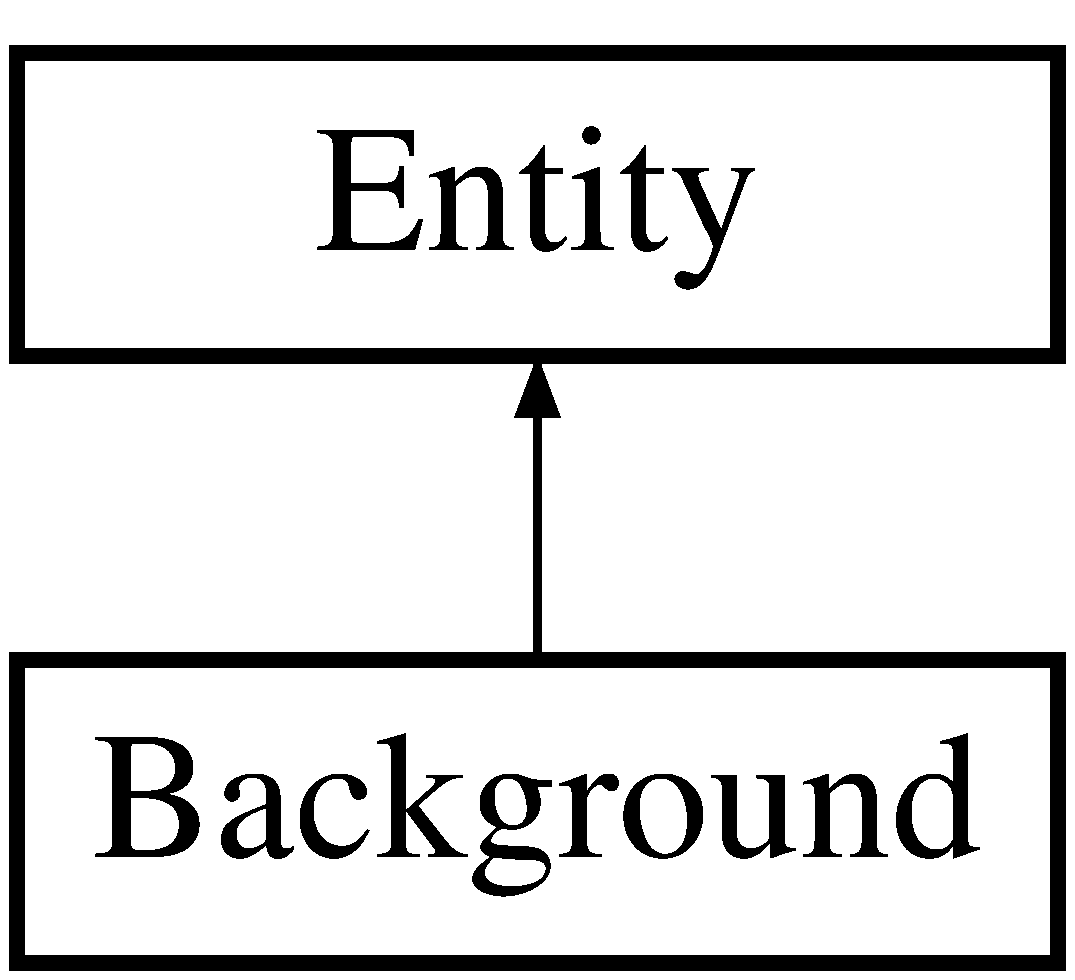
\includegraphics[height=2.000000cm]{class_background}
\end{center}
\end{figure}
\subsection*{Public Member Functions}
\begin{DoxyCompactItemize}
\item 
\hypertarget{class_background_a05b686e4ce0cbdb3b1fa14a93fdf98a1}{\hyperlink{class_background_a05b686e4ce0cbdb3b1fa14a93fdf98a1}{Background} ()}\label{class_background_a05b686e4ce0cbdb3b1fa14a93fdf98a1}

\begin{DoxyCompactList}\small\item\em sets mat\-I\-D to 0 for background \end{DoxyCompactList}\item 
\hypertarget{class_background_a688dc1ad4d16b9bc79966f7f71d40bb8}{\hyperlink{class_background_a688dc1ad4d16b9bc79966f7f71d40bb8}{$\sim$\-Background} ()=default}\label{class_background_a688dc1ad4d16b9bc79966f7f71d40bb8}

\begin{DoxyCompactList}\small\item\em default destructor \end{DoxyCompactList}\item 
\hypertarget{class_background_acab58b65d4299d4bd51b8376e8c3e3d3}{void \hyperlink{class_background_acab58b65d4299d4bd51b8376e8c3e3d3}{update} ()}\label{class_background_acab58b65d4299d4bd51b8376e8c3e3d3}

\begin{DoxyCompactList}\small\item\em update does nothing as quad is static \end{DoxyCompactList}\item 
\hypertarget{class_background_a448f05ff40a9d17be87c568294c63aaf}{void \hyperlink{class_background_a448f05ff40a9d17be87c568294c63aaf}{draw} ()}\label{class_background_a448f05ff40a9d17be87c568294c63aaf}

\begin{DoxyCompactList}\small\item\em draw the quad \end{DoxyCompactList}\item 
\hypertarget{class_background_ae07a9ea8891fdab015642386f77132c3}{void \hyperlink{class_background_ae07a9ea8891fdab015642386f77132c3}{create\-Quad} ()}\label{class_background_ae07a9ea8891fdab015642386f77132c3}

\begin{DoxyCompactList}\small\item\em initialise quad V\-A\-O \end{DoxyCompactList}\end{DoxyCompactItemize}
\subsection*{Private Attributes}
\begin{DoxyCompactItemize}
\item 
\hypertarget{class_background_a0a7b6b8f195c0e733a3fb8334137d32f}{G\-Luint \hyperlink{class_background_a0a7b6b8f195c0e733a3fb8334137d32f}{m\-\_\-vao\-I\-D}}\label{class_background_a0a7b6b8f195c0e733a3fb8334137d32f}

\begin{DoxyCompactList}\small\item\em identity of V\-A\-O \end{DoxyCompactList}\end{DoxyCompactItemize}
\subsection*{Additional Inherited Members}


\subsection{Detailed Description}
basically draws a quad fullscreen using whatever shader is set 

Definition at line 13 of file Background.\-h.



The documentation for this class was generated from the following files\-:\begin{DoxyCompactItemize}
\item 
C\-A1/i7621149-\/\-C\-A1/\-Final\-Submission/\-Template\-Project/include/\hyperlink{_background_8h}{Background.\-h}\item 
C\-A1/i7621149-\/\-C\-A1/\-Final\-Submission/\-Template\-Project/src/Background.\-cpp\end{DoxyCompactItemize}

\hypertarget{class_entity}{\section{Entity Class Reference}
\label{class_entity}\index{Entity@{Entity}}
}


this class contains everything the shader library needs to use it it also has information about position, rotation and scale, and functions to change the shader an instance uses  




{\ttfamily \#include $<$Entity.\-h$>$}

Inheritance diagram for Entity\-:\begin{figure}[H]
\begin{center}
\leavevmode
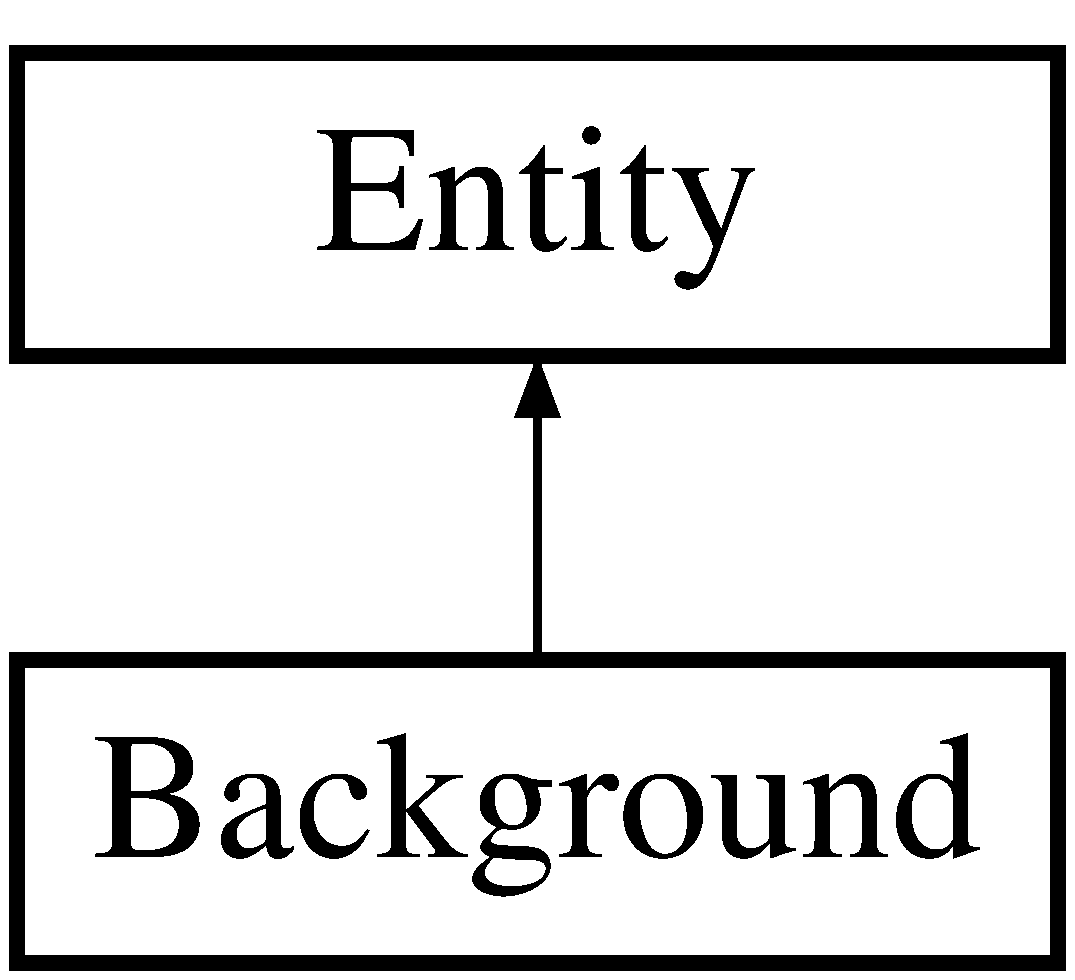
\includegraphics[height=2.000000cm]{class_entity}
\end{center}
\end{figure}
\subsection*{Public Member Functions}
\begin{DoxyCompactItemize}
\item 
\hyperlink{class_entity_a137651f62fa6c72984b83ff6c803fa37}{Entity} (int \-\_\-id, ngl\-::\-Vec3 \-\_\-pos)
\begin{DoxyCompactList}\small\item\em construct \hyperlink{class_entity}{Entity} with id and position, as well as set m\-\_\-alive to true \end{DoxyCompactList}\item 
\hypertarget{class_entity_aa6ecb9c57b29b60cc49fe44ad4088ecf}{\hyperlink{class_entity_aa6ecb9c57b29b60cc49fe44ad4088ecf}{$\sim$\-Entity} ()=default}\label{class_entity_aa6ecb9c57b29b60cc49fe44ad4088ecf}

\begin{DoxyCompactList}\small\item\em default destructor \end{DoxyCompactList}\item 
\hypertarget{class_entity_af4b2df22cccd334f7842055377ef45d2}{ngl\-::\-Mat4 \hyperlink{class_entity_af4b2df22cccd334f7842055377ef45d2}{get\-Transform\-Matrix} ()}\label{class_entity_af4b2df22cccd334f7842055377ef45d2}

\begin{DoxyCompactList}\small\item\em return transform matrix returns transform matrix of entity, based on pos, rot and scale \end{DoxyCompactList}\item 
ngl\-::\-Vec3 \hyperlink{class_entity_a644d5880f63b989fb975b7a999804e1b}{get\-Pos} ()
\begin{DoxyCompactList}\small\item\em get entity postion \end{DoxyCompactList}\item 
ngl\-::\-Vec3 \hyperlink{class_entity_aeaf9c87583d72c2d0b1b89275a747bc2}{get\-Vel} ()
\begin{DoxyCompactList}\small\item\em get entity velocity \end{DoxyCompactList}\item 
ngl\-::\-Vec3 \hyperlink{class_entity_add65f540d6cc42c97fe9552c7bb25c62}{get\-Rot} ()
\begin{DoxyCompactList}\small\item\em get entity rotation \end{DoxyCompactList}\item 
ngl\-::\-Vec3 \hyperlink{class_entity_aa74ac8c5835cafe7779efc39a2eaa8ce}{get\-Scale} ()
\begin{DoxyCompactList}\small\item\em get entity scale \end{DoxyCompactList}\item 
void \hyperlink{class_entity_a1c02a8d465e4c163168164cbf38da541}{set\-Pos} (ngl\-::\-Vec3 \-\_\-pos)
\begin{DoxyCompactList}\small\item\em set enitity position \end{DoxyCompactList}\item 
void \hyperlink{class_entity_a2b5fe9d66b26923a87fff92dbd6e63ed}{set\-Vel} (ngl\-::\-Vec3 \-\_\-vel)
\begin{DoxyCompactList}\small\item\em set entity velocity \end{DoxyCompactList}\item 
void \hyperlink{class_entity_a046b959de6e1306e5bcb8682e6623746}{set\-Rot} (ngl\-::\-Vec3 \-\_\-rot)
\begin{DoxyCompactList}\small\item\em set entity rotation \end{DoxyCompactList}\item 
void \hyperlink{class_entity_aebf26c8845b31f35104b91be523e84f9}{set\-Scale} (ngl\-::\-Vec3 \-\_\-scale)
\begin{DoxyCompactList}\small\item\em set entity scale \end{DoxyCompactList}\item 
int \hyperlink{class_entity_a00a43361a05770b2999ca90c612a159f}{get\-Shader\-Lib\-Index} ()
\begin{DoxyCompactList}\small\item\em return the current shader index the entity is using \end{DoxyCompactList}\item 
int \hyperlink{class_entity_a978bc19f08fed863dfb38d07f069430a}{get\-Current\-Index} ()
\begin{DoxyCompactList}\small\item\em return entity's current index \end{DoxyCompactList}\item 
void \hyperlink{class_entity_a26225c51294cbd3df67c53f29c6335b2}{set\-Current\-Index} (int \-\_\-index)
\begin{DoxyCompactList}\small\item\em set entity index \end{DoxyCompactList}\item 
void \hyperlink{class_entity_a4fa70ecbdba0609d08a6cb8d385031b1}{reset\-Index\-Range} (int \-\_\-min, int \-\_\-max)
\begin{DoxyCompactList}\small\item\em set the maximum and minimum shaders the shader can use \end{DoxyCompactList}\item 
int \hyperlink{class_entity_a1ccffcd9ad3ad9c44040ef7140758ddb}{get\-Min\-Index} ()
\begin{DoxyCompactList}\small\item\em find the minimum \hyperlink{class_shader_lib_pro}{Shader\-Lib\-Pro} index the entity can have \end{DoxyCompactList}\item 
int \hyperlink{class_entity_a6f4cf5bb25ba1210953d3d57130ce285}{get\-Max\-Index} ()
\begin{DoxyCompactList}\small\item\em find the maximum \hyperlink{class_shader_lib_pro}{Shader\-Lib\-Pro} index the entity can have \end{DoxyCompactList}\item 
int \hyperlink{class_entity_a6e158b373be07455338fd47823354c91}{get\-Mat\-I\-D} ()
\begin{DoxyCompactList}\small\item\em check the entity type \end{DoxyCompactList}\item 
bool \hyperlink{class_entity_ab0986ba7a1b24f022b5623781050c0f1}{is\-Alive} ()
\begin{DoxyCompactList}\small\item\em check if the entity is alive \end{DoxyCompactList}\item 
\hypertarget{class_entity_a59a29d9b7474baf13c9c76859242287d}{virtual void \hyperlink{class_entity_a59a29d9b7474baf13c9c76859242287d}{update} ()=0}\label{class_entity_a59a29d9b7474baf13c9c76859242287d}

\begin{DoxyCompactList}\small\item\em virtual update function to be overwritten \end{DoxyCompactList}\item 
\hypertarget{class_entity_a2e9a2986527958f0b0c43239efe9b270}{virtual void \hyperlink{class_entity_a2e9a2986527958f0b0c43239efe9b270}{draw} ()=0}\label{class_entity_a2e9a2986527958f0b0c43239efe9b270}

\begin{DoxyCompactList}\small\item\em virtual draw function to be overwritten \end{DoxyCompactList}\end{DoxyCompactItemize}
\subsection*{Protected Attributes}
\begin{DoxyCompactItemize}
\item 
\hypertarget{class_entity_a63fddde23301d8f868909fa77ea07d56}{int \hyperlink{class_entity_a63fddde23301d8f868909fa77ea07d56}{m\-\_\-mat\-I\-D}}\label{class_entity_a63fddde23301d8f868909fa77ea07d56}

\begin{DoxyCompactList}\small\item\em entity's material I\-D \end{DoxyCompactList}\item 
\hypertarget{class_entity_adc3eccf96ce5804512cd9d9a343d98f5}{ngl\-::\-Vec3 \hyperlink{class_entity_adc3eccf96ce5804512cd9d9a343d98f5}{m\-\_\-pos}}\label{class_entity_adc3eccf96ce5804512cd9d9a343d98f5}

\begin{DoxyCompactList}\small\item\em postion of entity \end{DoxyCompactList}\item 
\hypertarget{class_entity_ad2b217813dfbe55d39d6438b9b011d97}{ngl\-::\-Vec3 \hyperlink{class_entity_ad2b217813dfbe55d39d6438b9b011d97}{m\-\_\-vel} = ngl\-::\-Vec3(0,0,0)}\label{class_entity_ad2b217813dfbe55d39d6438b9b011d97}

\begin{DoxyCompactList}\small\item\em velocity of entity \end{DoxyCompactList}\item 
\hypertarget{class_entity_a7d345e8fda849e4f3f330289497c0955}{ngl\-::\-Vec3 \hyperlink{class_entity_a7d345e8fda849e4f3f330289497c0955}{m\-\_\-rot} = ngl\-::\-Vec3(0,0,0)}\label{class_entity_a7d345e8fda849e4f3f330289497c0955}

\begin{DoxyCompactList}\small\item\em rotation of entity \end{DoxyCompactList}\item 
\hypertarget{class_entity_a129334046e89817c024c29c81516843f}{ngl\-::\-Vec3 \hyperlink{class_entity_a129334046e89817c024c29c81516843f}{m\-\_\-scale} = ngl\-::\-Vec3(1,1,1)}\label{class_entity_a129334046e89817c024c29c81516843f}

\begin{DoxyCompactList}\small\item\em scale of entity \end{DoxyCompactList}\item 
\hypertarget{class_entity_a78efff1696f4c13a6f88b2fac836a02d}{int \hyperlink{class_entity_a78efff1696f4c13a6f88b2fac836a02d}{m\-\_\-current\-Index} = 0}\label{class_entity_a78efff1696f4c13a6f88b2fac836a02d}

\begin{DoxyCompactList}\small\item\em current shader index \end{DoxyCompactList}\item 
\hypertarget{class_entity_a93ac8660db956e864a33551c5f119026}{int \hyperlink{class_entity_a93ac8660db956e864a33551c5f119026}{m\-\_\-min\-Index} = 0}\label{class_entity_a93ac8660db956e864a33551c5f119026}

\begin{DoxyCompactList}\small\item\em minumum shader index allowed for entity \end{DoxyCompactList}\item 
\hypertarget{class_entity_ad053fa7e82312dad8e45f397ef857617}{int \hyperlink{class_entity_ad053fa7e82312dad8e45f397ef857617}{m\-\_\-max\-Index} = 99}\label{class_entity_ad053fa7e82312dad8e45f397ef857617}

\begin{DoxyCompactList}\small\item\em maximum shader index allowed for entity \end{DoxyCompactList}\item 
\hypertarget{class_entity_a0b7fba0256cc4275b4f326351d4750ca}{bool \hyperlink{class_entity_a0b7fba0256cc4275b4f326351d4750ca}{m\-\_\-alive}}\label{class_entity_a0b7fba0256cc4275b4f326351d4750ca}

\begin{DoxyCompactList}\small\item\em whether the entity is alive/active \end{DoxyCompactList}\end{DoxyCompactItemize}


\subsection{Detailed Description}
this class contains everything the shader library needs to use it it also has information about position, rotation and scale, and functions to change the shader an instance uses 

Definition at line 15 of file Entity.\-h.



\subsection{Constructor \& Destructor Documentation}
\hypertarget{class_entity_a137651f62fa6c72984b83ff6c803fa37}{\index{Entity@{Entity}!Entity@{Entity}}
\index{Entity@{Entity}!Entity@{Entity}}
\subsubsection[{Entity}]{\setlength{\rightskip}{0pt plus 5cm}Entity\-::\-Entity (
\begin{DoxyParamCaption}
\item[{int}]{\-\_\-id, }
\item[{ngl\-::\-Vec3}]{\-\_\-pos}
\end{DoxyParamCaption}
)}}\label{class_entity_a137651f62fa6c72984b83ff6c803fa37}


construct \hyperlink{class_entity}{Entity} with id and position, as well as set m\-\_\-alive to true 


\begin{DoxyParams}[1]{Parameters}
\mbox{\tt in}  & {\em \-\_\-id} & entity type, can be set by user and then used in shader \\
\hline
\mbox{\tt in}  & {\em \-\_\-pos} & initial position \\
\hline
\end{DoxyParams}


Definition at line 6 of file Entity.\-cpp.



\subsection{Member Function Documentation}
\hypertarget{class_entity_a978bc19f08fed863dfb38d07f069430a}{\index{Entity@{Entity}!get\-Current\-Index@{get\-Current\-Index}}
\index{get\-Current\-Index@{get\-Current\-Index}!Entity@{Entity}}
\subsubsection[{get\-Current\-Index}]{\setlength{\rightskip}{0pt plus 5cm}int Entity\-::get\-Current\-Index (
\begin{DoxyParamCaption}
{}
\end{DoxyParamCaption}
)\hspace{0.3cm}{\ttfamily [inline]}}}\label{class_entity_a978bc19f08fed863dfb38d07f069430a}


return entity's current index 

\begin{DoxyReturn}{Returns}
current index (relative to its minimum index) 
\end{DoxyReturn}


Definition at line 85 of file Entity.\-h.

\hypertarget{class_entity_a6e158b373be07455338fd47823354c91}{\index{Entity@{Entity}!get\-Mat\-I\-D@{get\-Mat\-I\-D}}
\index{get\-Mat\-I\-D@{get\-Mat\-I\-D}!Entity@{Entity}}
\subsubsection[{get\-Mat\-I\-D}]{\setlength{\rightskip}{0pt plus 5cm}int Entity\-::get\-Mat\-I\-D (
\begin{DoxyParamCaption}
{}
\end{DoxyParamCaption}
)\hspace{0.3cm}{\ttfamily [inline]}}}\label{class_entity_a6e158b373be07455338fd47823354c91}


check the entity type 

\begin{DoxyReturn}{Returns}
material id 
\end{DoxyReturn}


Definition at line 112 of file Entity.\-h.

\hypertarget{class_entity_a6f4cf5bb25ba1210953d3d57130ce285}{\index{Entity@{Entity}!get\-Max\-Index@{get\-Max\-Index}}
\index{get\-Max\-Index@{get\-Max\-Index}!Entity@{Entity}}
\subsubsection[{get\-Max\-Index}]{\setlength{\rightskip}{0pt plus 5cm}int Entity\-::get\-Max\-Index (
\begin{DoxyParamCaption}
{}
\end{DoxyParamCaption}
)\hspace{0.3cm}{\ttfamily [inline]}}}\label{class_entity_a6f4cf5bb25ba1210953d3d57130ce285}


find the maximum \hyperlink{class_shader_lib_pro}{Shader\-Lib\-Pro} index the entity can have 

\begin{DoxyReturn}{Returns}
the maximum index for \hyperlink{class_shader_lib_pro}{Shader\-Lib\-Pro} 
\end{DoxyReturn}


Definition at line 106 of file Entity.\-h.

\hypertarget{class_entity_a1ccffcd9ad3ad9c44040ef7140758ddb}{\index{Entity@{Entity}!get\-Min\-Index@{get\-Min\-Index}}
\index{get\-Min\-Index@{get\-Min\-Index}!Entity@{Entity}}
\subsubsection[{get\-Min\-Index}]{\setlength{\rightskip}{0pt plus 5cm}int Entity\-::get\-Min\-Index (
\begin{DoxyParamCaption}
{}
\end{DoxyParamCaption}
)\hspace{0.3cm}{\ttfamily [inline]}}}\label{class_entity_a1ccffcd9ad3ad9c44040ef7140758ddb}


find the minimum \hyperlink{class_shader_lib_pro}{Shader\-Lib\-Pro} index the entity can have 

\begin{DoxyReturn}{Returns}
the minimum index for \hyperlink{class_shader_lib_pro}{Shader\-Lib\-Pro} 
\end{DoxyReturn}


Definition at line 101 of file Entity.\-h.

\hypertarget{class_entity_a644d5880f63b989fb975b7a999804e1b}{\index{Entity@{Entity}!get\-Pos@{get\-Pos}}
\index{get\-Pos@{get\-Pos}!Entity@{Entity}}
\subsubsection[{get\-Pos}]{\setlength{\rightskip}{0pt plus 5cm}ngl\-::\-Vec3 Entity\-::get\-Pos (
\begin{DoxyParamCaption}
{}
\end{DoxyParamCaption}
)\hspace{0.3cm}{\ttfamily [inline]}}}\label{class_entity_a644d5880f63b989fb975b7a999804e1b}


get entity postion 

\begin{DoxyReturn}{Returns}
m\-\_\-pos 
\end{DoxyReturn}


Definition at line 38 of file Entity.\-h.

\hypertarget{class_entity_add65f540d6cc42c97fe9552c7bb25c62}{\index{Entity@{Entity}!get\-Rot@{get\-Rot}}
\index{get\-Rot@{get\-Rot}!Entity@{Entity}}
\subsubsection[{get\-Rot}]{\setlength{\rightskip}{0pt plus 5cm}ngl\-::\-Vec3 Entity\-::get\-Rot (
\begin{DoxyParamCaption}
{}
\end{DoxyParamCaption}
)\hspace{0.3cm}{\ttfamily [inline]}}}\label{class_entity_add65f540d6cc42c97fe9552c7bb25c62}


get entity rotation 

\begin{DoxyReturn}{Returns}
m\-\_\-rot 
\end{DoxyReturn}


Definition at line 48 of file Entity.\-h.

\hypertarget{class_entity_aa74ac8c5835cafe7779efc39a2eaa8ce}{\index{Entity@{Entity}!get\-Scale@{get\-Scale}}
\index{get\-Scale@{get\-Scale}!Entity@{Entity}}
\subsubsection[{get\-Scale}]{\setlength{\rightskip}{0pt plus 5cm}ngl\-::\-Vec3 Entity\-::get\-Scale (
\begin{DoxyParamCaption}
{}
\end{DoxyParamCaption}
)\hspace{0.3cm}{\ttfamily [inline]}}}\label{class_entity_aa74ac8c5835cafe7779efc39a2eaa8ce}


get entity scale 

\begin{DoxyReturn}{Returns}
m\-\_\-scale 
\end{DoxyReturn}


Definition at line 53 of file Entity.\-h.

\hypertarget{class_entity_a00a43361a05770b2999ca90c612a159f}{\index{Entity@{Entity}!get\-Shader\-Lib\-Index@{get\-Shader\-Lib\-Index}}
\index{get\-Shader\-Lib\-Index@{get\-Shader\-Lib\-Index}!Entity@{Entity}}
\subsubsection[{get\-Shader\-Lib\-Index}]{\setlength{\rightskip}{0pt plus 5cm}int Entity\-::get\-Shader\-Lib\-Index (
\begin{DoxyParamCaption}
{}
\end{DoxyParamCaption}
)\hspace{0.3cm}{\ttfamily [inline]}}}\label{class_entity_a00a43361a05770b2999ca90c612a159f}


return the current shader index the entity is using 

\begin{DoxyReturn}{Returns}
shader index for \hyperlink{class_shader_lib_pro}{Shader\-Lib\-Pro} 
\end{DoxyReturn}


Definition at line 80 of file Entity.\-h.

\hypertarget{class_entity_aeaf9c87583d72c2d0b1b89275a747bc2}{\index{Entity@{Entity}!get\-Vel@{get\-Vel}}
\index{get\-Vel@{get\-Vel}!Entity@{Entity}}
\subsubsection[{get\-Vel}]{\setlength{\rightskip}{0pt plus 5cm}ngl\-::\-Vec3 Entity\-::get\-Vel (
\begin{DoxyParamCaption}
{}
\end{DoxyParamCaption}
)\hspace{0.3cm}{\ttfamily [inline]}}}\label{class_entity_aeaf9c87583d72c2d0b1b89275a747bc2}


get entity velocity 

\begin{DoxyReturn}{Returns}
m\-\_\-vel 
\end{DoxyReturn}


Definition at line 43 of file Entity.\-h.

\hypertarget{class_entity_ab0986ba7a1b24f022b5623781050c0f1}{\index{Entity@{Entity}!is\-Alive@{is\-Alive}}
\index{is\-Alive@{is\-Alive}!Entity@{Entity}}
\subsubsection[{is\-Alive}]{\setlength{\rightskip}{0pt plus 5cm}bool Entity\-::is\-Alive (
\begin{DoxyParamCaption}
{}
\end{DoxyParamCaption}
)\hspace{0.3cm}{\ttfamily [inline]}}}\label{class_entity_ab0986ba7a1b24f022b5623781050c0f1}


check if the entity is alive 

\begin{DoxyReturn}{Returns}
whether the entity is alive 
\end{DoxyReturn}


Definition at line 118 of file Entity.\-h.

\hypertarget{class_entity_a4fa70ecbdba0609d08a6cb8d385031b1}{\index{Entity@{Entity}!reset\-Index\-Range@{reset\-Index\-Range}}
\index{reset\-Index\-Range@{reset\-Index\-Range}!Entity@{Entity}}
\subsubsection[{reset\-Index\-Range}]{\setlength{\rightskip}{0pt plus 5cm}void Entity\-::reset\-Index\-Range (
\begin{DoxyParamCaption}
\item[{int}]{\-\_\-min, }
\item[{int}]{\-\_\-max}
\end{DoxyParamCaption}
)}}\label{class_entity_a4fa70ecbdba0609d08a6cb8d385031b1}


set the maximum and minimum shaders the shader can use 


\begin{DoxyParams}[1]{Parameters}
\mbox{\tt in}  & {\em \-\_\-min} & the minimum index for \hyperlink{class_shader_lib_pro}{Shader\-Lib\-Pro} \\
\hline
\mbox{\tt in}  & {\em \-\_\-max} & the maximum index for \hyperlink{class_shader_lib_pro}{Shader\-Lib\-Pro} \\
\hline
\end{DoxyParams}


Definition at line 24 of file Entity.\-cpp.

\hypertarget{class_entity_a26225c51294cbd3df67c53f29c6335b2}{\index{Entity@{Entity}!set\-Current\-Index@{set\-Current\-Index}}
\index{set\-Current\-Index@{set\-Current\-Index}!Entity@{Entity}}
\subsubsection[{set\-Current\-Index}]{\setlength{\rightskip}{0pt plus 5cm}void Entity\-::set\-Current\-Index (
\begin{DoxyParamCaption}
\item[{int}]{\-\_\-index}
\end{DoxyParamCaption}
)}}\label{class_entity_a26225c51294cbd3df67c53f29c6335b2}


set entity index 


\begin{DoxyParams}[1]{Parameters}
\mbox{\tt in}  & {\em index} & (relative to its minimum index, eg input 0 to get its minimum) \\
\hline
\end{DoxyParams}


Definition at line 32 of file Entity.\-cpp.

\hypertarget{class_entity_a1c02a8d465e4c163168164cbf38da541}{\index{Entity@{Entity}!set\-Pos@{set\-Pos}}
\index{set\-Pos@{set\-Pos}!Entity@{Entity}}
\subsubsection[{set\-Pos}]{\setlength{\rightskip}{0pt plus 5cm}void Entity\-::set\-Pos (
\begin{DoxyParamCaption}
\item[{ngl\-::\-Vec3}]{\-\_\-pos}
\end{DoxyParamCaption}
)\hspace{0.3cm}{\ttfamily [inline]}}}\label{class_entity_a1c02a8d465e4c163168164cbf38da541}


set enitity position 


\begin{DoxyParams}[1]{Parameters}
\mbox{\tt in}  & {\em \-\_\-pos} & postion \\
\hline
\end{DoxyParams}


Definition at line 59 of file Entity.\-h.

\hypertarget{class_entity_a046b959de6e1306e5bcb8682e6623746}{\index{Entity@{Entity}!set\-Rot@{set\-Rot}}
\index{set\-Rot@{set\-Rot}!Entity@{Entity}}
\subsubsection[{set\-Rot}]{\setlength{\rightskip}{0pt plus 5cm}void Entity\-::set\-Rot (
\begin{DoxyParamCaption}
\item[{ngl\-::\-Vec3}]{\-\_\-rot}
\end{DoxyParamCaption}
)\hspace{0.3cm}{\ttfamily [inline]}}}\label{class_entity_a046b959de6e1306e5bcb8682e6623746}


set entity rotation 


\begin{DoxyParams}[1]{Parameters}
\mbox{\tt in}  & {\em \-\_\-rot} & rotation \\
\hline
\end{DoxyParams}


Definition at line 69 of file Entity.\-h.

\hypertarget{class_entity_aebf26c8845b31f35104b91be523e84f9}{\index{Entity@{Entity}!set\-Scale@{set\-Scale}}
\index{set\-Scale@{set\-Scale}!Entity@{Entity}}
\subsubsection[{set\-Scale}]{\setlength{\rightskip}{0pt plus 5cm}void Entity\-::set\-Scale (
\begin{DoxyParamCaption}
\item[{ngl\-::\-Vec3}]{\-\_\-scale}
\end{DoxyParamCaption}
)\hspace{0.3cm}{\ttfamily [inline]}}}\label{class_entity_aebf26c8845b31f35104b91be523e84f9}


set entity scale 


\begin{DoxyParams}[1]{Parameters}
\mbox{\tt in}  & {\em \-\_\-scale} & scale \\
\hline
\end{DoxyParams}


Definition at line 74 of file Entity.\-h.

\hypertarget{class_entity_a2b5fe9d66b26923a87fff92dbd6e63ed}{\index{Entity@{Entity}!set\-Vel@{set\-Vel}}
\index{set\-Vel@{set\-Vel}!Entity@{Entity}}
\subsubsection[{set\-Vel}]{\setlength{\rightskip}{0pt plus 5cm}void Entity\-::set\-Vel (
\begin{DoxyParamCaption}
\item[{ngl\-::\-Vec3}]{\-\_\-vel}
\end{DoxyParamCaption}
)\hspace{0.3cm}{\ttfamily [inline]}}}\label{class_entity_a2b5fe9d66b26923a87fff92dbd6e63ed}


set entity velocity 


\begin{DoxyParams}[1]{Parameters}
\mbox{\tt in}  & {\em \-\_\-vel} & velocity \\
\hline
\end{DoxyParams}


Definition at line 64 of file Entity.\-h.



The documentation for this class was generated from the following files\-:\begin{DoxyCompactItemize}
\item 
C\-A1/i7621149-\/\-C\-A1/\-Final\-Submission/\-Template\-Project/include/\hyperlink{_entity_8h}{Entity.\-h}\item 
C\-A1/i7621149-\/\-C\-A1/\-Final\-Submission/\-Template\-Project/src/Entity.\-cpp\end{DoxyCompactItemize}

\hypertarget{class_n_g_l_scene}{\section{N\-G\-L\-Scene Class Reference}
\label{class_n_g_l_scene}\index{N\-G\-L\-Scene@{N\-G\-L\-Scene}}
}


this contains the major management and drawing functions of our programs  




{\ttfamily \#include $<$N\-G\-L\-Scene.\-h$>$}

Inheritance diagram for N\-G\-L\-Scene\-:\begin{figure}[H]
\begin{center}
\leavevmode
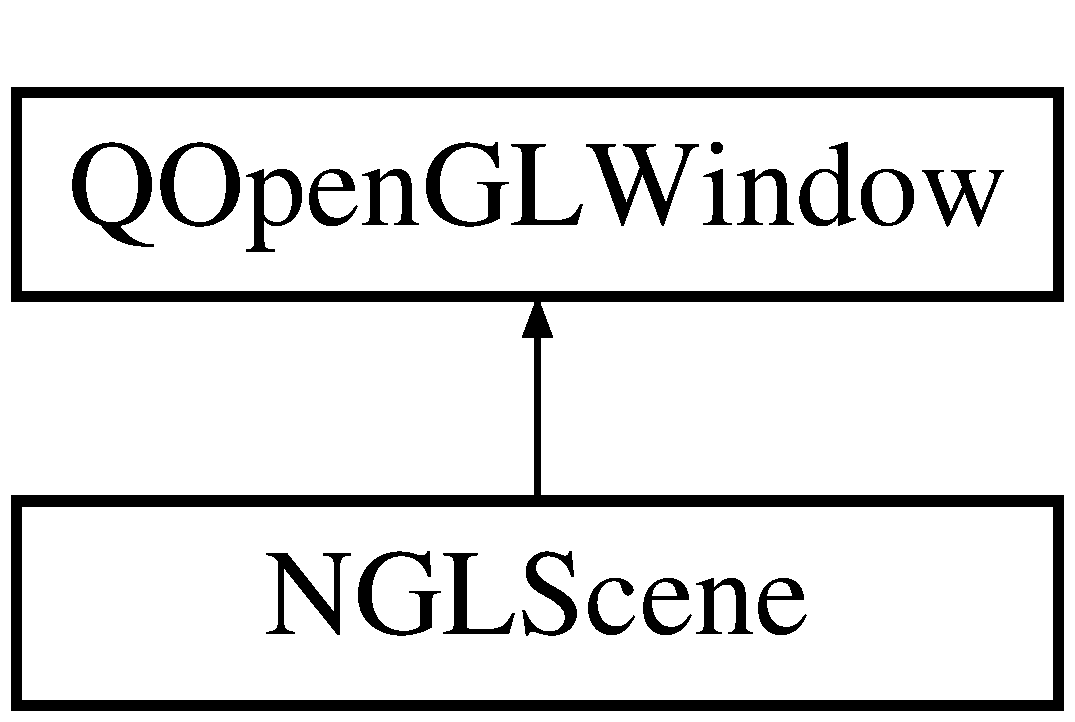
\includegraphics[height=2.000000cm]{class_n_g_l_scene}
\end{center}
\end{figure}
\subsection*{Public Member Functions}
\begin{DoxyCompactItemize}
\item 
\hypertarget{class_n_g_l_scene_a1bed6be9823459aeb1e58af2464ba633}{\hyperlink{class_n_g_l_scene_a1bed6be9823459aeb1e58af2464ba633}{N\-G\-L\-Scene} ()}\label{class_n_g_l_scene_a1bed6be9823459aeb1e58af2464ba633}

\begin{DoxyCompactList}\small\item\em initialise variables not dependent on Open\-G\-L or ngl \end{DoxyCompactList}\item 
\hypertarget{class_n_g_l_scene_abda05d130945833bfbb6bad8d619f7f5}{\hyperlink{class_n_g_l_scene_abda05d130945833bfbb6bad8d619f7f5}{$\sim$\-N\-G\-L\-Scene} ()}\label{class_n_g_l_scene_abda05d130945833bfbb6bad8d619f7f5}

\begin{DoxyCompactList}\small\item\em destructor prints message \end{DoxyCompactList}\end{DoxyCompactItemize}
\subsection*{Private Member Functions}
\begin{DoxyCompactItemize}
\item 
\hypertarget{class_n_g_l_scene_aab2b866db534d286a56cc2240ed98790}{void \hyperlink{class_n_g_l_scene_aab2b866db534d286a56cc2240ed98790}{initialize\-G\-L} ()}\label{class_n_g_l_scene_aab2b866db534d286a56cc2240ed98790}

\begin{DoxyCompactList}\small\item\em initialise shaders and variables etc, after initialising ngl \end{DoxyCompactList}\item 
\hypertarget{class_n_g_l_scene_a37bec65bfba7b7a717d803d369221e2d}{void \hyperlink{class_n_g_l_scene_a37bec65bfba7b7a717d803d369221e2d}{paint\-G\-L} ()}\label{class_n_g_l_scene_a37bec65bfba7b7a717d803d369221e2d}

\begin{DoxyCompactList}\small\item\em render scene, called upon update(), which is called in timer\-Event \end{DoxyCompactList}\item 
void \hyperlink{class_n_g_l_scene_a39f61e86b1e5a6c8125e3a762ea3f7f7}{resize\-G\-L} (Q\-Resize\-Event $\ast$\-\_\-event)
\begin{DoxyCompactList}\small\item\em called upon resizing window \end{DoxyCompactList}\item 
void \hyperlink{class_n_g_l_scene_a7505fac688fe82b4f99e601043eb7764}{resize\-G\-L} (int \-\_\-w, int \-\_\-h)
\begin{DoxyCompactList}\small\item\em called upon resizing window \end{DoxyCompactList}\item 
void \hyperlink{class_n_g_l_scene_a7a03bd8f485d27c4de72d24139ed8f8a}{key\-Press\-Event} (Q\-Key\-Event $\ast$\-\_\-event)
\begin{DoxyCompactList}\small\item\em called upon hitting a key \end{DoxyCompactList}\item 
void \hyperlink{class_n_g_l_scene_abfb1a790affff40de7183fa4016d1d2b}{key\-Release\-Event} (Q\-Key\-Event $\ast$\-\_\-event)
\begin{DoxyCompactList}\small\item\em called upon releasing a key \end{DoxyCompactList}\item 
void \hyperlink{class_n_g_l_scene_aa9822d94cb9c93a666fef86d86d2cf6c}{mouse\-Move\-Event} (Q\-Mouse\-Event $\ast$\-\_\-event)
\begin{DoxyCompactList}\small\item\em called upon moving the mouse \end{DoxyCompactList}\item 
void \hyperlink{class_n_g_l_scene_a8ead414be695622f8ace373628a25727}{mouse\-Press\-Event} (Q\-Mouse\-Event $\ast$\-\_\-event)
\begin{DoxyCompactList}\small\item\em called upon pressing the mouse \end{DoxyCompactList}\item 
void \hyperlink{class_n_g_l_scene_a6f363e63153342d91bafd3bdaf271c20}{mouse\-Release\-Event} (Q\-Mouse\-Event $\ast$\-\_\-event)
\begin{DoxyCompactList}\small\item\em called upon releasing the mouse \end{DoxyCompactList}\item 
void \hyperlink{class_n_g_l_scene_a5ea289b6eb36df76da5e6e39be04c779}{wheel\-Event} (Q\-Wheel\-Event $\ast$\-\_\-event)
\begin{DoxyCompactList}\small\item\em called upon scrolling \end{DoxyCompactList}\item 
void \hyperlink{class_n_g_l_scene_afeb250f7c7b1cac320d06dd14a279cb9}{timer\-Event} (Q\-Timer\-Event $\ast$\-\_\-event)
\begin{DoxyCompactList}\small\item\em called every timer event \end{DoxyCompactList}\item 
\hypertarget{class_n_g_l_scene_ab9cff1e645aa573a5679a55e5c845da8}{void \hyperlink{class_n_g_l_scene_ab9cff1e645aa573a5679a55e5c845da8}{toggle\-Full\-Screen} ()}\label{class_n_g_l_scene_ab9cff1e645aa573a5679a55e5c845da8}

\begin{DoxyCompactList}\small\item\em toggle program between normal and fullscreen \end{DoxyCompactList}\end{DoxyCompactItemize}
\subsection*{Private Attributes}
\begin{DoxyCompactItemize}
\item 
\hypertarget{class_n_g_l_scene_a8d5dabddc30ca59d34088595bdd7d174}{int \hyperlink{class_n_g_l_scene_a8d5dabddc30ca59d34088595bdd7d174}{m\-\_\-width}}\label{class_n_g_l_scene_a8d5dabddc30ca59d34088595bdd7d174}

\begin{DoxyCompactList}\small\item\em screen width \end{DoxyCompactList}\item 
\hypertarget{class_n_g_l_scene_ad0fccff55fd9df6af9adda2c654de21d}{int \hyperlink{class_n_g_l_scene_ad0fccff55fd9df6af9adda2c654de21d}{m\-\_\-height}}\label{class_n_g_l_scene_ad0fccff55fd9df6af9adda2c654de21d}

\begin{DoxyCompactList}\small\item\em screen height \end{DoxyCompactList}\item 
\hypertarget{class_n_g_l_scene_a969d56f1bfb80598b0333107bb1fb60c}{bool \hyperlink{class_n_g_l_scene_a969d56f1bfb80598b0333107bb1fb60c}{m\-\_\-full\-Screen}}\label{class_n_g_l_scene_a969d56f1bfb80598b0333107bb1fb60c}

\begin{DoxyCompactList}\small\item\em whether program is in fullscreen mode \end{DoxyCompactList}\item 
\hypertarget{class_n_g_l_scene_ab5830b16af87f2843e8f41d212a6eb01}{bool \hyperlink{class_n_g_l_scene_ab5830b16af87f2843e8f41d212a6eb01}{m\-\_\-mouse\-Down}}\label{class_n_g_l_scene_ab5830b16af87f2843e8f41d212a6eb01}

\begin{DoxyCompactList}\small\item\em whether mouse is pressed \end{DoxyCompactList}\item 
\hypertarget{class_n_g_l_scene_a9de69b584317b729b6fd95d1bcc37f05}{Q\-Time \hyperlink{class_n_g_l_scene_a9de69b584317b729b6fd95d1bcc37f05}{m\-\_\-time}}\label{class_n_g_l_scene_a9de69b584317b729b6fd95d1bcc37f05}

\begin{DoxyCompactList}\small\item\em used to check elapsed time, set to time of program start \end{DoxyCompactList}\item 
\hypertarget{class_n_g_l_scene_a043c90078e0862126109544a5fe24b33}{int \hyperlink{class_n_g_l_scene_a043c90078e0862126109544a5fe24b33}{m\-\_\-last\-Frame\-Time}}\label{class_n_g_l_scene_a043c90078e0862126109544a5fe24b33}

\begin{DoxyCompactList}\small\item\em milliseconds taken to render last frame \end{DoxyCompactList}\item 
\hypertarget{class_n_g_l_scene_af270fda48df0e58b244f0484f8d3ad2d}{ngl\-::\-Vec4 \hyperlink{class_n_g_l_scene_af270fda48df0e58b244f0484f8d3ad2d}{m\-\_\-mouse\-Data}}\label{class_n_g_l_scene_af270fda48df0e58b244f0484f8d3ad2d}

\begin{DoxyCompactList}\small\item\em mouse data. x, y\-: mouse position if m\-\_\-mouse\-Down (else last position when m\-\_\-mouse\-Down) z, w\-: initial mouse position on click (if mouse is up, is negative) \end{DoxyCompactList}\item 
\hypertarget{class_n_g_l_scene_a4faea2adadeaad479ff774e8345815e6}{ngl\-::\-Camera \hyperlink{class_n_g_l_scene_a4faea2adadeaad479ff774e8345815e6}{m\-\_\-cam}}\label{class_n_g_l_scene_a4faea2adadeaad479ff774e8345815e6}

\begin{DoxyCompactList}\small\item\em scene camera \end{DoxyCompactList}\item 
\hypertarget{class_n_g_l_scene_aa72ef89c47d7b79a65cd07227ed6bb17}{\hyperlink{class_background}{Background} \hyperlink{class_n_g_l_scene_aa72ef89c47d7b79a65cd07227ed6bb17}{m\-\_\-background}}\label{class_n_g_l_scene_aa72ef89c47d7b79a65cd07227ed6bb17}

\begin{DoxyCompactList}\small\item\em background entity, single quad \end{DoxyCompactList}\end{DoxyCompactItemize}


\subsection{Detailed Description}
this contains the major management and drawing functions of our programs 

Definition at line 23 of file N\-G\-L\-Scene.\-h.



\subsection{Member Function Documentation}
\hypertarget{class_n_g_l_scene_a7a03bd8f485d27c4de72d24139ed8f8a}{\index{N\-G\-L\-Scene@{N\-G\-L\-Scene}!key\-Press\-Event@{key\-Press\-Event}}
\index{key\-Press\-Event@{key\-Press\-Event}!NGLScene@{N\-G\-L\-Scene}}
\subsubsection[{key\-Press\-Event}]{\setlength{\rightskip}{0pt plus 5cm}void N\-G\-L\-Scene\-::key\-Press\-Event (
\begin{DoxyParamCaption}
\item[{Q\-Key\-Event $\ast$}]{\-\_\-event}
\end{DoxyParamCaption}
)\hspace{0.3cm}{\ttfamily [private]}}}\label{class_n_g_l_scene_a7a03bd8f485d27c4de72d24139ed8f8a}


called upon hitting a key 


\begin{DoxyParams}[1]{Parameters}
\mbox{\tt in}  & {\em \-\_\-event} & Qt key event containing key info, such as type \\
\hline
\end{DoxyParams}


Definition at line 138 of file N\-G\-L\-Scene.\-cpp.

\hypertarget{class_n_g_l_scene_abfb1a790affff40de7183fa4016d1d2b}{\index{N\-G\-L\-Scene@{N\-G\-L\-Scene}!key\-Release\-Event@{key\-Release\-Event}}
\index{key\-Release\-Event@{key\-Release\-Event}!NGLScene@{N\-G\-L\-Scene}}
\subsubsection[{key\-Release\-Event}]{\setlength{\rightskip}{0pt plus 5cm}void N\-G\-L\-Scene\-::key\-Release\-Event (
\begin{DoxyParamCaption}
\item[{Q\-Key\-Event $\ast$}]{\-\_\-event}
\end{DoxyParamCaption}
)\hspace{0.3cm}{\ttfamily [private]}}}\label{class_n_g_l_scene_abfb1a790affff40de7183fa4016d1d2b}


called upon releasing a key 


\begin{DoxyParams}[1]{Parameters}
\mbox{\tt in}  & {\em \-\_\-event} & Qt key event containing key info, such as type \\
\hline
\end{DoxyParams}


Definition at line 158 of file N\-G\-L\-Scene.\-cpp.

\hypertarget{class_n_g_l_scene_aa9822d94cb9c93a666fef86d86d2cf6c}{\index{N\-G\-L\-Scene@{N\-G\-L\-Scene}!mouse\-Move\-Event@{mouse\-Move\-Event}}
\index{mouse\-Move\-Event@{mouse\-Move\-Event}!NGLScene@{N\-G\-L\-Scene}}
\subsubsection[{mouse\-Move\-Event}]{\setlength{\rightskip}{0pt plus 5cm}void N\-G\-L\-Scene\-::mouse\-Move\-Event (
\begin{DoxyParamCaption}
\item[{Q\-Mouse\-Event $\ast$}]{\-\_\-event}
\end{DoxyParamCaption}
)\hspace{0.3cm}{\ttfamily [private]}}}\label{class_n_g_l_scene_aa9822d94cb9c93a666fef86d86d2cf6c}


called upon moving the mouse 


\begin{DoxyParams}[1]{Parameters}
\mbox{\tt in}  & {\em \-\_\-event} & Qt mouse event containing mouse position etc \\
\hline
\end{DoxyParams}


Definition at line 107 of file N\-G\-L\-Scene.\-cpp.

\hypertarget{class_n_g_l_scene_a8ead414be695622f8ace373628a25727}{\index{N\-G\-L\-Scene@{N\-G\-L\-Scene}!mouse\-Press\-Event@{mouse\-Press\-Event}}
\index{mouse\-Press\-Event@{mouse\-Press\-Event}!NGLScene@{N\-G\-L\-Scene}}
\subsubsection[{mouse\-Press\-Event}]{\setlength{\rightskip}{0pt plus 5cm}void N\-G\-L\-Scene\-::mouse\-Press\-Event (
\begin{DoxyParamCaption}
\item[{Q\-Mouse\-Event $\ast$}]{\-\_\-event}
\end{DoxyParamCaption}
)\hspace{0.3cm}{\ttfamily [private]}}}\label{class_n_g_l_scene_a8ead414be695622f8ace373628a25727}


called upon pressing the mouse 


\begin{DoxyParams}[1]{Parameters}
\mbox{\tt in}  & {\em \-\_\-event} & Qt mouse event containing mouse position etc \\
\hline
\end{DoxyParams}


Definition at line 117 of file N\-G\-L\-Scene.\-cpp.

\hypertarget{class_n_g_l_scene_a6f363e63153342d91bafd3bdaf271c20}{\index{N\-G\-L\-Scene@{N\-G\-L\-Scene}!mouse\-Release\-Event@{mouse\-Release\-Event}}
\index{mouse\-Release\-Event@{mouse\-Release\-Event}!NGLScene@{N\-G\-L\-Scene}}
\subsubsection[{mouse\-Release\-Event}]{\setlength{\rightskip}{0pt plus 5cm}void N\-G\-L\-Scene\-::mouse\-Release\-Event (
\begin{DoxyParamCaption}
\item[{Q\-Mouse\-Event $\ast$}]{\-\_\-event}
\end{DoxyParamCaption}
)\hspace{0.3cm}{\ttfamily [private]}}}\label{class_n_g_l_scene_a6f363e63153342d91bafd3bdaf271c20}


called upon releasing the mouse 


\begin{DoxyParams}[1]{Parameters}
\mbox{\tt in}  & {\em \-\_\-event} & Qt mouse event containing mouse position etc \\
\hline
\end{DoxyParams}


Definition at line 125 of file N\-G\-L\-Scene.\-cpp.

\hypertarget{class_n_g_l_scene_a39f61e86b1e5a6c8125e3a762ea3f7f7}{\index{N\-G\-L\-Scene@{N\-G\-L\-Scene}!resize\-G\-L@{resize\-G\-L}}
\index{resize\-G\-L@{resize\-G\-L}!NGLScene@{N\-G\-L\-Scene}}
\subsubsection[{resize\-G\-L}]{\setlength{\rightskip}{0pt plus 5cm}void N\-G\-L\-Scene\-::resize\-G\-L (
\begin{DoxyParamCaption}
\item[{Q\-Resize\-Event $\ast$}]{\-\_\-event}
\end{DoxyParamCaption}
)\hspace{0.3cm}{\ttfamily [private]}}}\label{class_n_g_l_scene_a39f61e86b1e5a6c8125e3a762ea3f7f7}


called upon resizing window 


\begin{DoxyParams}[1]{Parameters}
\mbox{\tt in}  & {\em \-\_\-event} & Qt resize event containing new width and height \\
\hline
\end{DoxyParams}


Definition at line 32 of file N\-G\-L\-Scene.\-cpp.

\hypertarget{class_n_g_l_scene_a7505fac688fe82b4f99e601043eb7764}{\index{N\-G\-L\-Scene@{N\-G\-L\-Scene}!resize\-G\-L@{resize\-G\-L}}
\index{resize\-G\-L@{resize\-G\-L}!NGLScene@{N\-G\-L\-Scene}}
\subsubsection[{resize\-G\-L}]{\setlength{\rightskip}{0pt plus 5cm}void N\-G\-L\-Scene\-::resize\-G\-L (
\begin{DoxyParamCaption}
\item[{int}]{\-\_\-w, }
\item[{int}]{\-\_\-h}
\end{DoxyParamCaption}
)\hspace{0.3cm}{\ttfamily [private]}}}\label{class_n_g_l_scene_a7505fac688fe82b4f99e601043eb7764}


called upon resizing window 


\begin{DoxyParams}[1]{Parameters}
\mbox{\tt in}  & {\em \-\_\-w} & width of window \\
\hline
\mbox{\tt in}  & {\em \-\_\-h} & height of window \\
\hline
\end{DoxyParams}


Definition at line 43 of file N\-G\-L\-Scene.\-cpp.

\hypertarget{class_n_g_l_scene_afeb250f7c7b1cac320d06dd14a279cb9}{\index{N\-G\-L\-Scene@{N\-G\-L\-Scene}!timer\-Event@{timer\-Event}}
\index{timer\-Event@{timer\-Event}!NGLScene@{N\-G\-L\-Scene}}
\subsubsection[{timer\-Event}]{\setlength{\rightskip}{0pt plus 5cm}void N\-G\-L\-Scene\-::timer\-Event (
\begin{DoxyParamCaption}
\item[{Q\-Timer\-Event $\ast$}]{\-\_\-event}
\end{DoxyParamCaption}
)\hspace{0.3cm}{\ttfamily [private]}}}\label{class_n_g_l_scene_afeb250f7c7b1cac320d06dd14a279cb9}


called every timer event 


\begin{DoxyParams}[1]{Parameters}
\mbox{\tt in}  & {\em \-\_\-event} & Qt timer event, can be used if multiple timers are set up \\
\hline
\end{DoxyParams}


Definition at line 163 of file N\-G\-L\-Scene.\-cpp.

\hypertarget{class_n_g_l_scene_a5ea289b6eb36df76da5e6e39be04c779}{\index{N\-G\-L\-Scene@{N\-G\-L\-Scene}!wheel\-Event@{wheel\-Event}}
\index{wheel\-Event@{wheel\-Event}!NGLScene@{N\-G\-L\-Scene}}
\subsubsection[{wheel\-Event}]{\setlength{\rightskip}{0pt plus 5cm}void N\-G\-L\-Scene\-::wheel\-Event (
\begin{DoxyParamCaption}
\item[{Q\-Wheel\-Event $\ast$}]{\-\_\-event}
\end{DoxyParamCaption}
)\hspace{0.3cm}{\ttfamily [private]}}}\label{class_n_g_l_scene_a5ea289b6eb36df76da5e6e39be04c779}


called upon scrolling 


\begin{DoxyParams}[1]{Parameters}
\mbox{\tt in}  & {\em \-\_\-event} & Qt mousewheel event \\
\hline
\end{DoxyParams}


Definition at line 133 of file N\-G\-L\-Scene.\-cpp.



The documentation for this class was generated from the following files\-:\begin{DoxyCompactItemize}
\item 
C\-A1/i7621149-\/\-C\-A1/\-Final\-Submission/\-Template\-Project/include/\hyperlink{_n_g_l_scene_8h}{N\-G\-L\-Scene.\-h}\item 
C\-A1/i7621149-\/\-C\-A1/\-Final\-Submission/\-Template\-Project/src/N\-G\-L\-Scene.\-cpp\end{DoxyCompactItemize}

\hypertarget{class_shader_lib_pro}{\section{Shader\-Lib\-Pro Class Reference}
\label{class_shader_lib_pro}\index{Shader\-Lib\-Pro@{Shader\-Lib\-Pro}}
}
Inheritance diagram for Shader\-Lib\-Pro\-:\begin{figure}[H]
\begin{center}
\leavevmode
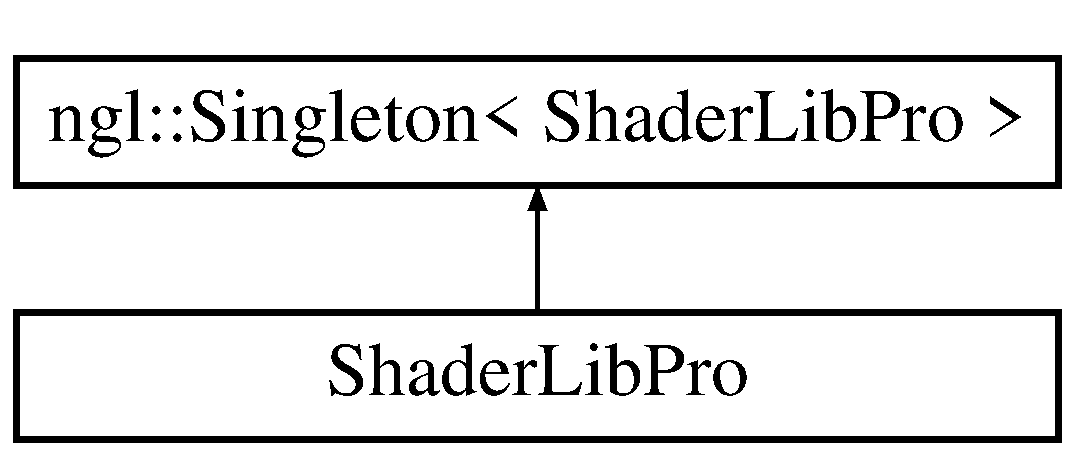
\includegraphics[height=2.000000cm]{class_shader_lib_pro}
\end{center}
\end{figure}
\subsection*{Public Member Functions}
\begin{DoxyCompactItemize}
\item 
void \hyperlink{class_shader_lib_pro_a7a12f281cef251008a3ccbc04fd2fb52}{add\-Shader} (const std\-::string \&\-\_\-source\-File)
\begin{DoxyCompactList}\small\item\em add a \hyperlink{class_shader_set}{Shader\-Set} to the library, loaded from text file \end{DoxyCompactList}\item 
void \hyperlink{class_shader_lib_pro_ae7059e210cd4fc739d12209e904dea75}{draw} (\hyperlink{class_entity}{Entity} $\ast$\-\_\-entity, ngl\-::\-Camera $\ast$\-\_\-cam)
\begin{DoxyCompactList}\small\item\em draw an entity \end{DoxyCompactList}\item 
void \hyperlink{class_shader_lib_pro_a9401ba0fe34177ba6955ce769cec1f9b}{use\-Shader} (size\-\_\-t \-\_\-index)
\begin{DoxyCompactList}\small\item\em use a specific shader, specified when drawing, by the entity \end{DoxyCompactList}\item 
int \hyperlink{class_shader_lib_pro_a16e8698616a023de15e48b8107d2d1d4}{get\-Shader\-Set\-Amount} ()
\begin{DoxyCompactList}\small\item\em find out how many Shader\-Sets there currently are \end{DoxyCompactList}\end{DoxyCompactItemize}
\subsection*{Private Member Functions}
\begin{DoxyCompactItemize}
\item 
\hypertarget{class_shader_lib_pro_a69c266b5eabde43b4ca472f36489a1ef}{\hyperlink{class_shader_lib_pro_a69c266b5eabde43b4ca472f36489a1ef}{Shader\-Lib\-Pro} ()}\label{class_shader_lib_pro_a69c266b5eabde43b4ca472f36489a1ef}

\begin{DoxyCompactList}\small\item\em constructor initialises m\-\_\-shader\-Sets and m\-\_\-current\-Shader\-Index to 0 \end{DoxyCompactList}\item 
\hypertarget{class_shader_lib_pro_a78b250ffc06b58d1a6de95ccadead58d}{\hyperlink{class_shader_lib_pro_a78b250ffc06b58d1a6de95ccadead58d}{$\sim$\-Shader\-Lib\-Pro} ()}\label{class_shader_lib_pro_a78b250ffc06b58d1a6de95ccadead58d}

\begin{DoxyCompactList}\small\item\em destructor prints message to std\-::cout \end{DoxyCompactList}\end{DoxyCompactItemize}
\subsection*{Private Attributes}
\begin{DoxyCompactItemize}
\item 
\hypertarget{class_shader_lib_pro_ab5415f8247ca7df067ad212ed624cd29}{std\-::vector$<$ std\-::unique\-\_\-ptr\\*
$<$ \hyperlink{class_shader_set}{Shader\-Set} $>$ $>$ \hyperlink{class_shader_lib_pro_ab5415f8247ca7df067ad212ed624cd29}{m\-\_\-shader\-Sets}}\label{class_shader_lib_pro_ab5415f8247ca7df067ad212ed624cd29}

\begin{DoxyCompactList}\small\item\em vector of Shader\-Sets currently active \end{DoxyCompactList}\item 
\hypertarget{class_shader_lib_pro_a14c11ed244083ea9e82f8e040ba684b9}{int \hyperlink{class_shader_lib_pro_a14c11ed244083ea9e82f8e040ba684b9}{m\-\_\-current\-Shaderindex}}\label{class_shader_lib_pro_a14c11ed244083ea9e82f8e040ba684b9}

\begin{DoxyCompactList}\small\item\em current shader being used \end{DoxyCompactList}\end{DoxyCompactItemize}
\subsection*{Friends}
\begin{DoxyCompactItemize}
\item 
\hypertarget{class_shader_lib_pro_ae3463efce7974572eefeef5e31732375}{class {\bfseries ngl\-::\-Singleton$<$ Shader\-Lib\-Pro $>$}}\label{class_shader_lib_pro_ae3463efce7974572eefeef5e31732375}

\end{DoxyCompactItemize}


\subsection{Detailed Description}


Definition at line 20 of file Shader\-Lib\-Pro.\-h.



\subsection{Member Function Documentation}
\hypertarget{class_shader_lib_pro_a7a12f281cef251008a3ccbc04fd2fb52}{\index{Shader\-Lib\-Pro@{Shader\-Lib\-Pro}!add\-Shader@{add\-Shader}}
\index{add\-Shader@{add\-Shader}!ShaderLibPro@{Shader\-Lib\-Pro}}
\subsubsection[{add\-Shader}]{\setlength{\rightskip}{0pt plus 5cm}void Shader\-Lib\-Pro\-::add\-Shader (
\begin{DoxyParamCaption}
\item[{const std\-::string \&}]{\-\_\-source\-File}
\end{DoxyParamCaption}
)}}\label{class_shader_lib_pro_a7a12f281cef251008a3ccbc04fd2fb52}


add a \hyperlink{class_shader_set}{Shader\-Set} to the library, loaded from text file 


\begin{DoxyParams}[1]{Parameters}
\mbox{\tt in}  & {\em \-\_\-source\-File} & text file to source shader from \\
\hline
\end{DoxyParams}


Definition at line 36 of file Shader\-Lib\-Pro.\-cpp.

\hypertarget{class_shader_lib_pro_ae7059e210cd4fc739d12209e904dea75}{\index{Shader\-Lib\-Pro@{Shader\-Lib\-Pro}!draw@{draw}}
\index{draw@{draw}!ShaderLibPro@{Shader\-Lib\-Pro}}
\subsubsection[{draw}]{\setlength{\rightskip}{0pt plus 5cm}void Shader\-Lib\-Pro\-::draw (
\begin{DoxyParamCaption}
\item[{{\bf Entity} $\ast$}]{\-\_\-entity, }
\item[{ngl\-::\-Camera $\ast$}]{\-\_\-cam}
\end{DoxyParamCaption}
)}}\label{class_shader_lib_pro_ae7059e210cd4fc739d12209e904dea75}


draw an entity 


\begin{DoxyParams}[1]{Parameters}
\mbox{\tt in}  & {\em \-\_\-entity} & the entity to draw \\
\hline
\mbox{\tt in}  & {\em \-\_\-cam} & camera to draw from, can be nullptr to use identity matrices \\
\hline
\end{DoxyParams}


Definition at line 41 of file Shader\-Lib\-Pro.\-cpp.

\hypertarget{class_shader_lib_pro_a16e8698616a023de15e48b8107d2d1d4}{\index{Shader\-Lib\-Pro@{Shader\-Lib\-Pro}!get\-Shader\-Set\-Amount@{get\-Shader\-Set\-Amount}}
\index{get\-Shader\-Set\-Amount@{get\-Shader\-Set\-Amount}!ShaderLibPro@{Shader\-Lib\-Pro}}
\subsubsection[{get\-Shader\-Set\-Amount}]{\setlength{\rightskip}{0pt plus 5cm}int Shader\-Lib\-Pro\-::get\-Shader\-Set\-Amount (
\begin{DoxyParamCaption}
{}
\end{DoxyParamCaption}
)\hspace{0.3cm}{\ttfamily [inline]}}}\label{class_shader_lib_pro_a16e8698616a023de15e48b8107d2d1d4}


find out how many Shader\-Sets there currently are 

\begin{DoxyReturn}{Returns}
number of shaders 
\end{DoxyReturn}


Definition at line 45 of file Shader\-Lib\-Pro.\-h.

\hypertarget{class_shader_lib_pro_a9401ba0fe34177ba6955ce769cec1f9b}{\index{Shader\-Lib\-Pro@{Shader\-Lib\-Pro}!use\-Shader@{use\-Shader}}
\index{use\-Shader@{use\-Shader}!ShaderLibPro@{Shader\-Lib\-Pro}}
\subsubsection[{use\-Shader}]{\setlength{\rightskip}{0pt plus 5cm}void Shader\-Lib\-Pro\-::use\-Shader (
\begin{DoxyParamCaption}
\item[{size\-\_\-t}]{\-\_\-index}
\end{DoxyParamCaption}
)}}\label{class_shader_lib_pro_a9401ba0fe34177ba6955ce769cec1f9b}


use a specific shader, specified when drawing, by the entity 


\begin{DoxyParams}[1]{Parameters}
\mbox{\tt in}  & {\em \-\_\-index} & the index of the shader to use \\
\hline
\end{DoxyParams}


Definition at line 23 of file Shader\-Lib\-Pro.\-cpp.



The documentation for this class was generated from the following files\-:\begin{DoxyCompactItemize}
\item 
C\-A1/i7621149-\/\-C\-A1/\-Final\-Submission/\-Template\-Project/include/\hyperlink{_shader_lib_pro_8h}{Shader\-Lib\-Pro.\-h}\item 
C\-A1/i7621149-\/\-C\-A1/\-Final\-Submission/\-Template\-Project/src/Shader\-Lib\-Pro.\-cpp\end{DoxyCompactItemize}

\hypertarget{struct_shader_pro}{\section{Shader\-Pro Struct Reference}
\label{struct_shader_pro}\index{Shader\-Pro@{Shader\-Pro}}
}


mostly used to add shaders and use shaders. simple interaction means it is easy to use  




{\ttfamily \#include $<$Shader\-Lib\-Pro.\-h$>$}

\subsection*{Public Types}
\begin{DoxyCompactItemize}
\item 
enum \hyperlink{struct_shader_pro_a1dfb06c4b3b2d1651492a0a3c44ef555}{Debug\-Mode} \{ {\bfseries C\-O\-M\-P\-I\-L\-E}, 
{\bfseries L\-I\-N\-K}
 \}
\begin{DoxyCompactList}\small\item\em enum used for debugging \end{DoxyCompactList}\end{DoxyCompactItemize}
\subsection*{Public Member Functions}
\begin{DoxyCompactItemize}
\item 
\hypertarget{struct_shader_pro_a6a156214f2ccce2b6995cd27b1489e8e}{\hyperlink{struct_shader_pro_a6a156214f2ccce2b6995cd27b1489e8e}{Shader\-Pro} ()}\label{struct_shader_pro_a6a156214f2ccce2b6995cd27b1489e8e}

\begin{DoxyCompactList}\small\item\em contructor initialises values to 0 \end{DoxyCompactList}\item 
\hypertarget{struct_shader_pro_a5a188aa3f9272f910d0911da07ce131d}{\hyperlink{struct_shader_pro_a5a188aa3f9272f910d0911da07ce131d}{$\sim$\-Shader\-Pro} ()}\label{struct_shader_pro_a5a188aa3f9272f910d0911da07ce131d}

\begin{DoxyCompactList}\small\item\em destructor deletes framebuffers \end{DoxyCompactList}\item 
\hypertarget{struct_shader_pro_a4044a4eac55f3a13b7bffc932dc6b980}{void \hyperlink{struct_shader_pro_a4044a4eac55f3a13b7bffc932dc6b980}{compile} ()}\label{struct_shader_pro_a4044a4eac55f3a13b7bffc932dc6b980}

\begin{DoxyCompactList}\small\item\em compile the source code to be used by the shader library \end{DoxyCompactList}\item 
\hypertarget{struct_shader_pro_abe5d4cf1c8eb0457e022a9b4df208056}{void \hyperlink{struct_shader_pro_abe5d4cf1c8eb0457e022a9b4df208056}{load\-Vert\-Source} ()}\label{struct_shader_pro_abe5d4cf1c8eb0457e022a9b4df208056}

\begin{DoxyCompactList}\small\item\em load source code for the vertex shader, including adding the Base\-Vertex code \end{DoxyCompactList}\item 
\hypertarget{struct_shader_pro_a1b91bc81ec80f37ee9ff9145a6604272}{void \hyperlink{struct_shader_pro_a1b91bc81ec80f37ee9ff9145a6604272}{load\-Frag\-Source} ()}\label{struct_shader_pro_a1b91bc81ec80f37ee9ff9145a6604272}

\begin{DoxyCompactList}\small\item\em load source code for the frag shader, including adding the Base\-Vertex code \end{DoxyCompactList}\item 
std\-::string \hyperlink{struct_shader_pro_a07d7c40d47452a9b5b108854398a27bc}{load\-Source} (const std\-::string \&\-\_\-file\-Name)
\begin{DoxyCompactList}\small\item\em loads text from a file \end{DoxyCompactList}\item 
std\-::string \hyperlink{struct_shader_pro_a2597c8fede9842fad4b0e14db042ef91}{get\-Frag\-Base} ()
\begin{DoxyCompactList}\small\item\em load fragment base code to add to fragment glsl file \end{DoxyCompactList}\item 
\hypertarget{struct_shader_pro_a20ab79316be828c3d08f5016739e48a5}{void \hyperlink{struct_shader_pro_a20ab79316be828c3d08f5016739e48a5}{load\-Textures} ()}\label{struct_shader_pro_a20ab79316be828c3d08f5016739e48a5}

\begin{DoxyCompactList}\small\item\em load the textures from their source files \end{DoxyCompactList}\item 
\hypertarget{struct_shader_pro_ad54d2cce5d4fac7089610de3602fc2af}{void \hyperlink{struct_shader_pro_ad54d2cce5d4fac7089610de3602fc2af}{textures\-To\-Shader} ()}\label{struct_shader_pro_ad54d2cce5d4fac7089610de3602fc2af}

\begin{DoxyCompactList}\small\item\em link the textures to the shader \end{DoxyCompactList}\item 
void \hyperlink{struct_shader_pro_a641844c63583b896ecc5822a17eef21b}{load\-Image} (int \-\_\-texture\-Unit, \hyperlink{struct_texture_data}{Texture\-Data} \-\_\-texture, G\-Lenum \-\_\-type)
\begin{DoxyCompactList}\small\item\em read an image from a file to a Gl texture \end{DoxyCompactList}\item 
\hypertarget{struct_shader_pro_a2d111c2168ed1c32f622a14f7d8dceaf}{void \hyperlink{struct_shader_pro_a2d111c2168ed1c32f622a14f7d8dceaf}{print\-Shader\-Data} ()}\label{struct_shader_pro_a2d111c2168ed1c32f622a14f7d8dceaf}

\begin{DoxyCompactList}\small\item\em prints most values contained within the shader, useful for debugging \end{DoxyCompactList}\item 
\hypertarget{struct_shader_pro_a055b4e00dff7becc620096b74ada78f5}{void \hyperlink{struct_shader_pro_a055b4e00dff7becc620096b74ada78f5}{print\-Info\-Log} (G\-Luint \-\_\-id, \hyperlink{struct_shader_pro_a1dfb06c4b3b2d1651492a0a3c44ef555}{Debug\-Mode} \-\_\-mode)}\label{struct_shader_pro_a055b4e00dff7becc620096b74ada78f5}

\begin{DoxyCompactList}\small\item\em prints info from shader compile, for checking errors \end{DoxyCompactList}\item 
\hypertarget{struct_shader_pro_a0c4bf7215d8c134752b13a9a86842ba2}{void \hyperlink{struct_shader_pro_a0c4bf7215d8c134752b13a9a86842ba2}{set\-Up\-Framebuffer} ()}\label{struct_shader_pro_a0c4bf7215d8c134752b13a9a86842ba2}

\begin{DoxyCompactList}\small\item\em creates data required for frame buffer (still in progress) \end{DoxyCompactList}\end{DoxyCompactItemize}
\subsection*{Public Attributes}
\begin{DoxyCompactItemize}
\item 
\hypertarget{struct_shader_pro_a5f134047e932f52e46d1bde8eccc447c}{std\-::string \hyperlink{struct_shader_pro_a5f134047e932f52e46d1bde8eccc447c}{m\-\_\-name}}\label{struct_shader_pro_a5f134047e932f52e46d1bde8eccc447c}

\begin{DoxyCompactList}\small\item\em name given to shader in text file, eg \char`\"{}\-M\-A\-I\-N\char`\"{} \end{DoxyCompactList}\item 
\hypertarget{struct_shader_pro_a129da0c17bbe478c3e3d53cab7015d02}{G\-Luint \hyperlink{struct_shader_pro_a129da0c17bbe478c3e3d53cab7015d02}{m\-\_\-prog\-I\-D}}\label{struct_shader_pro_a129da0c17bbe478c3e3d53cab7015d02}

\begin{DoxyCompactList}\small\item\em shader program I\-D, used by open\-G\-L \end{DoxyCompactList}\item 
\hypertarget{struct_shader_pro_aef7140b201165a62e77216fd8479f094}{G\-Luint \hyperlink{struct_shader_pro_aef7140b201165a62e77216fd8479f094}{m\-\_\-frag\-I\-D}}\label{struct_shader_pro_aef7140b201165a62e77216fd8479f094}

\begin{DoxyCompactList}\small\item\em fragment shader I\-D \end{DoxyCompactList}\item 
\hypertarget{struct_shader_pro_ab798c7c102d4183fc36392884374aaee}{G\-Luint \hyperlink{struct_shader_pro_ab798c7c102d4183fc36392884374aaee}{m\-\_\-vert\-I\-D}}\label{struct_shader_pro_ab798c7c102d4183fc36392884374aaee}

\begin{DoxyCompactList}\small\item\em vertex shader I\-D \end{DoxyCompactList}\item 
\hypertarget{struct_shader_pro_aedfab2d94289b844c81ec90b94e337b5}{G\-Luint \hyperlink{struct_shader_pro_aedfab2d94289b844c81ec90b94e337b5}{m\-\_\-out\-Buffer\-I\-D}}\label{struct_shader_pro_aedfab2d94289b844c81ec90b94e337b5}

\begin{DoxyCompactList}\small\item\em framebuffer I\-D, if it has one, otherwise is set to 0 \end{DoxyCompactList}\item 
\hypertarget{struct_shader_pro_a710261840d8482d848970b1b8967f828}{G\-Luint \hyperlink{struct_shader_pro_a710261840d8482d848970b1b8967f828}{m\-\_\-out\-Texture\-I\-D}}\label{struct_shader_pro_a710261840d8482d848970b1b8967f828}

\begin{DoxyCompactList}\small\item\em texture I\-D coming out if it renders to a framebuffer \end{DoxyCompactList}\item 
\hypertarget{struct_shader_pro_a604a470b247093aa492537ce53f41442}{G\-Luint \hyperlink{struct_shader_pro_a604a470b247093aa492537ce53f41442}{m\-\_\-out\-Depth\-Stencil\-I\-D}}\label{struct_shader_pro_a604a470b247093aa492537ce53f41442}

\begin{DoxyCompactList}\small\item\em out depth stencil id, used for rendering to a frame buffer \end{DoxyCompactList}\item 
\hypertarget{struct_shader_pro_a29aae1d3375fa42b3c78b1cb035e2675}{std\-::string \hyperlink{struct_shader_pro_a29aae1d3375fa42b3c78b1cb035e2675}{m\-\_\-frag\-File}}\label{struct_shader_pro_a29aae1d3375fa42b3c78b1cb035e2675}

\begin{DoxyCompactList}\small\item\em source file of frament shader \end{DoxyCompactList}\item 
\hypertarget{struct_shader_pro_aea0734e5aa1dc6ddf7b7bdd20f235848}{std\-::string \hyperlink{struct_shader_pro_aea0734e5aa1dc6ddf7b7bdd20f235848}{m\-\_\-vert\-File}}\label{struct_shader_pro_aea0734e5aa1dc6ddf7b7bdd20f235848}

\begin{DoxyCompactList}\small\item\em source file of vertex shader \end{DoxyCompactList}\item 
\hypertarget{struct_shader_pro_afa957000f293f2fb4217f28f0db321ec}{std\-::vector$<$ \hyperlink{struct_texture_data}{Texture\-Data} $>$ \hyperlink{struct_shader_pro_afa957000f293f2fb4217f28f0db321ec}{m\-\_\-textures}}\label{struct_shader_pro_afa957000f293f2fb4217f28f0db321ec}

\begin{DoxyCompactList}\small\item\em vector of \hyperlink{struct_texture_data}{Texture\-Data} structs \end{DoxyCompactList}\end{DoxyCompactItemize}


\subsection{Detailed Description}
mostly used to add shaders and use shaders. simple interaction means it is easy to use 

\hyperlink{struct_shader_pro}{Shader\-Pro} seems complex but this allows the data to be managed away from a user. It does a lot for the user such as loading source, linking and compiling. 

Definition at line 19 of file Shader\-Pro.\-h.



\subsection{Member Function Documentation}
\hypertarget{struct_shader_pro_a2597c8fede9842fad4b0e14db042ef91}{\index{Shader\-Pro@{Shader\-Pro}!get\-Frag\-Base@{get\-Frag\-Base}}
\index{get\-Frag\-Base@{get\-Frag\-Base}!ShaderPro@{Shader\-Pro}}
\subsubsection[{get\-Frag\-Base}]{\setlength{\rightskip}{0pt plus 5cm}std\-::string Shader\-Pro\-::get\-Frag\-Base (
\begin{DoxyParamCaption}
{}
\end{DoxyParamCaption}
)}}\label{struct_shader_pro_a2597c8fede9842fad4b0e14db042ef91}


load fragment base code to add to fragment glsl file 

\begin{DoxyReturn}{Returns}
the text from the file as well as any texture uniforms required 
\end{DoxyReturn}


Definition at line 103 of file Shader\-Pro.\-cpp.

\hypertarget{struct_shader_pro_a641844c63583b896ecc5822a17eef21b}{\index{Shader\-Pro@{Shader\-Pro}!load\-Image@{load\-Image}}
\index{load\-Image@{load\-Image}!ShaderPro@{Shader\-Pro}}
\subsubsection[{load\-Image}]{\setlength{\rightskip}{0pt plus 5cm}void Shader\-Pro\-::load\-Image (
\begin{DoxyParamCaption}
\item[{int}]{\-\_\-texture\-Unit, }
\item[{{\bf Texture\-Data}}]{\-\_\-texture, }
\item[{G\-Lenum}]{\-\_\-type}
\end{DoxyParamCaption}
)}}\label{struct_shader_pro_a641844c63583b896ecc5822a17eef21b}


read an image from a file to a Gl texture 


\begin{DoxyParams}[1]{Parameters}
\mbox{\tt in}  & {\em \-\_\-texture\-Unit} & the texture number, eg 0, 1, 2 as shaders can have multiple textures \\
\hline
\mbox{\tt in}  & {\em \-\_\-texture} & struct containing all information of the shader \\
\hline
\mbox{\tt in}  & {\em \-\_\-type} & the type of shader to load, all G\-L\-\_\-\-T\-E\-X\-T\-U\-R\-E\-\_\-2\-D at the moment \\
\hline
\end{DoxyParams}


Definition at line 185 of file Shader\-Pro.\-cpp.

\hypertarget{struct_shader_pro_a07d7c40d47452a9b5b108854398a27bc}{\index{Shader\-Pro@{Shader\-Pro}!load\-Source@{load\-Source}}
\index{load\-Source@{load\-Source}!ShaderPro@{Shader\-Pro}}
\subsubsection[{load\-Source}]{\setlength{\rightskip}{0pt plus 5cm}std\-::string Shader\-Pro\-::load\-Source (
\begin{DoxyParamCaption}
\item[{const std\-::string \&}]{\-\_\-file\-Name}
\end{DoxyParamCaption}
)}}\label{struct_shader_pro_a07d7c40d47452a9b5b108854398a27bc}


loads text from a file 


\begin{DoxyParams}[1]{Parameters}
\mbox{\tt in}  & {\em \-\_\-file\-Name} & the text file containing data for a shader \\
\hline
\end{DoxyParams}
\begin{DoxyReturn}{Returns}
the text from the file 
\end{DoxyReturn}


Definition at line 85 of file Shader\-Pro.\-cpp.



The documentation for this struct was generated from the following files\-:\begin{DoxyCompactItemize}
\item 
C\-A1/i7621149-\/\-C\-A1/\-Final\-Submission/\-Template\-Project/include/\hyperlink{_shader_pro_8h}{Shader\-Pro.\-h}\item 
C\-A1/i7621149-\/\-C\-A1/\-Final\-Submission/\-Template\-Project/src/Shader\-Pro.\-cpp\end{DoxyCompactItemize}

\hypertarget{class_shader_set}{\section{Shader\-Set Class Reference}
\label{class_shader_set}\index{Shader\-Set@{Shader\-Set}}
}


Shader\-Sets contain a vector of shaders and are responsible for managing them and making draw calls to Entities.  




{\ttfamily \#include $<$Shader\-Set.\-h$>$}

\subsection*{Public Member Functions}
\begin{DoxyCompactItemize}
\item 
\hyperlink{class_shader_set_a9bbabbd777c8ca13efb7d8b1d919fb11}{Shader\-Set} (const std\-::string \&\-\_\-source\-File)
\begin{DoxyCompactList}\small\item\em constructor from source file, taken in text form (see report) \end{DoxyCompactList}\item 
\hypertarget{class_shader_set_a026cd1988dbd45e6e7e061b2d92d8fbd}{\hyperlink{class_shader_set_a026cd1988dbd45e6e7e061b2d92d8fbd}{$\sim$\-Shader\-Set} ()=default}\label{class_shader_set_a026cd1988dbd45e6e7e061b2d92d8fbd}

\begin{DoxyCompactList}\small\item\em default destructor \end{DoxyCompactList}\item 
void \hyperlink{class_shader_set_aede001dacb08e161768755e9018d0d12}{set\-Shader\-Info} (const std\-::string \&\-\_\-source\-File)
\begin{DoxyCompactList}\small\item\em used in constructor to read source file and generate shader vector \end{DoxyCompactList}\item 
void \hyperlink{class_shader_set_adc30a6cd9c60ac29c6a103f60d9b4929}{draw} (\hyperlink{class_entity}{Entity} $\ast$\-\_\-entity, ngl\-::\-Camera $\ast$\-\_\-cam)
\begin{DoxyCompactList}\small\item\em draw the inputted entity \end{DoxyCompactList}\item 
\hypertarget{class_shader_set_a716a9bdfc98bd1c43f3c07bbf8b492b8}{void \hyperlink{class_shader_set_a716a9bdfc98bd1c43f3c07bbf8b492b8}{load\-Shaders} ()}\label{class_shader_set_a716a9bdfc98bd1c43f3c07bbf8b492b8}

\begin{DoxyCompactList}\small\item\em compiles all shaders \end{DoxyCompactList}\item 
\hyperlink{struct_shader_pro}{Shader\-Pro} $\ast$ \hyperlink{class_shader_set_af4fe473c04f2707865df20496723b1e7}{get\-Shader} (const std\-::string \&\-\_\-shader\-Name)
\begin{DoxyCompactList}\small\item\em return pointer to shader referred to \end{DoxyCompactList}\end{DoxyCompactItemize}
\subsection*{Private Attributes}
\begin{DoxyCompactItemize}
\item 
\hypertarget{class_shader_set_ad0da5edb6d6dfd043ebf9a2551f12346}{std\-::vector$<$ std\-::unique\-\_\-ptr\\*
$<$ \hyperlink{struct_shader_pro}{Shader\-Pro} $>$ $>$ \hyperlink{class_shader_set_ad0da5edb6d6dfd043ebf9a2551f12346}{m\-\_\-shaders}}\label{class_shader_set_ad0da5edb6d6dfd043ebf9a2551f12346}

\begin{DoxyCompactList}\small\item\em vector of unique pointers to shaders in the set \end{DoxyCompactList}\end{DoxyCompactItemize}


\subsection{Detailed Description}
Shader\-Sets contain a vector of shaders and are responsible for managing them and making draw calls to Entities. 

Definition at line 18 of file Shader\-Set.\-h.



\subsection{Constructor \& Destructor Documentation}
\hypertarget{class_shader_set_a9bbabbd777c8ca13efb7d8b1d919fb11}{\index{Shader\-Set@{Shader\-Set}!Shader\-Set@{Shader\-Set}}
\index{Shader\-Set@{Shader\-Set}!ShaderSet@{Shader\-Set}}
\subsubsection[{Shader\-Set}]{\setlength{\rightskip}{0pt plus 5cm}Shader\-Set\-::\-Shader\-Set (
\begin{DoxyParamCaption}
\item[{const std\-::string \&}]{\-\_\-source\-File}
\end{DoxyParamCaption}
)}}\label{class_shader_set_a9bbabbd777c8ca13efb7d8b1d919fb11}


constructor from source file, taken in text form (see report) 


\begin{DoxyParams}[1]{Parameters}
\mbox{\tt in}  & {\em \-\_\-source\-File} & the text file to read in a shader \\
\hline
\end{DoxyParams}


Definition at line 11 of file Shader\-Set.\-cpp.



\subsection{Member Function Documentation}
\hypertarget{class_shader_set_adc30a6cd9c60ac29c6a103f60d9b4929}{\index{Shader\-Set@{Shader\-Set}!draw@{draw}}
\index{draw@{draw}!ShaderSet@{Shader\-Set}}
\subsubsection[{draw}]{\setlength{\rightskip}{0pt plus 5cm}void Shader\-Set\-::draw (
\begin{DoxyParamCaption}
\item[{{\bf Entity} $\ast$}]{\-\_\-entity, }
\item[{ngl\-::\-Camera $\ast$}]{\-\_\-cam}
\end{DoxyParamCaption}
)}}\label{class_shader_set_adc30a6cd9c60ac29c6a103f60d9b4929}


draw the inputted entity 


\begin{DoxyParams}[1]{Parameters}
\mbox{\tt in}  & {\em \-\_\-entity} & the entity to draw \\
\hline
\mbox{\tt in}  & {\em \-\_\-cam} & the camera to use for M\-V\-P etc \\
\hline
\end{DoxyParams}


Definition at line 220 of file Shader\-Set.\-cpp.

\hypertarget{class_shader_set_af4fe473c04f2707865df20496723b1e7}{\index{Shader\-Set@{Shader\-Set}!get\-Shader@{get\-Shader}}
\index{get\-Shader@{get\-Shader}!ShaderSet@{Shader\-Set}}
\subsubsection[{get\-Shader}]{\setlength{\rightskip}{0pt plus 5cm}{\bf Shader\-Pro} $\ast$ Shader\-Set\-::get\-Shader (
\begin{DoxyParamCaption}
\item[{const std\-::string \&}]{\-\_\-shader\-Name}
\end{DoxyParamCaption}
)}}\label{class_shader_set_af4fe473c04f2707865df20496723b1e7}


return pointer to shader referred to 


\begin{DoxyParams}[1]{Parameters}
\mbox{\tt in}  & {\em \-\_\-shader\-Name} & the name given to the shader from the text file, eg \char`\"{}\-M\-A\-I\-N\char`\"{} \\
\hline
\end{DoxyParams}
\begin{DoxyReturn}{Returns}
pointer to the shader needed 
\end{DoxyReturn}


Definition at line 277 of file Shader\-Set.\-cpp.

\hypertarget{class_shader_set_aede001dacb08e161768755e9018d0d12}{\index{Shader\-Set@{Shader\-Set}!set\-Shader\-Info@{set\-Shader\-Info}}
\index{set\-Shader\-Info@{set\-Shader\-Info}!ShaderSet@{Shader\-Set}}
\subsubsection[{set\-Shader\-Info}]{\setlength{\rightskip}{0pt plus 5cm}void Shader\-Set\-::set\-Shader\-Info (
\begin{DoxyParamCaption}
\item[{const std\-::string \&}]{\-\_\-source\-File}
\end{DoxyParamCaption}
)}}\label{class_shader_set_aede001dacb08e161768755e9018d0d12}


used in constructor to read source file and generate shader vector 


\begin{DoxyParams}[1]{Parameters}
\mbox{\tt in}  & {\em \-\_\-source\-File} & the text file to read in a shader \\
\hline
\end{DoxyParams}


Definition at line 18 of file Shader\-Set.\-cpp.



The documentation for this class was generated from the following files\-:\begin{DoxyCompactItemize}
\item 
C\-A1/i7621149-\/\-C\-A1/\-Final\-Submission/\-Template\-Project/include/\hyperlink{_shader_set_8h}{Shader\-Set.\-h}\item 
C\-A1/i7621149-\/\-C\-A1/\-Final\-Submission/\-Template\-Project/src/Shader\-Set.\-cpp\end{DoxyCompactItemize}

\hypertarget{struct_shader_variables}{\section{Shader\-Variables Struct Reference}
\label{struct_shader_variables}\index{Shader\-Variables@{Shader\-Variables}}
}


This contains variables passed to the shader as uniforms, such as resolution, time, rendertime, frame number, mouse data and date it also contains the current material id and transform matrix its member variables are public for ease of use.  




{\ttfamily \#include $<$Shader\-Variables.\-h$>$}

Inheritance diagram for Shader\-Variables\-:\begin{figure}[H]
\begin{center}
\leavevmode
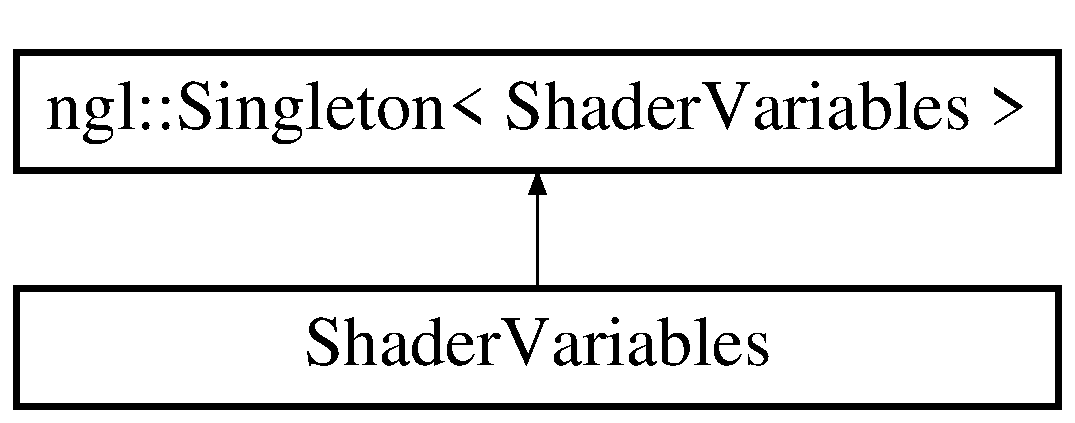
\includegraphics[height=2.000000cm]{struct_shader_variables}
\end{center}
\end{figure}
\subsection*{Public Member Functions}
\begin{DoxyCompactItemize}
\item 
void \hyperlink{struct_shader_variables_a6c4056a98de2375814f543ac22b5f7a4}{reset} (bool \-\_\-hard=false)
\begin{DoxyCompactList}\small\item\em reset values in the shader \end{DoxyCompactList}\item 
void \hyperlink{struct_shader_variables_a47ff8143a673b365033858fa1acc3d10}{load\-To\-Shader} (G\-Luint \-\_\-prog\-I\-D)
\begin{DoxyCompactList}\small\item\em load the variables to the shader program \end{DoxyCompactList}\item 
\hypertarget{struct_shader_variables_a022653bc55d573feb772b1502949ad8e}{void \hyperlink{struct_shader_variables_a022653bc55d573feb772b1502949ad8e}{print\-Variables} ()}\label{struct_shader_variables_a022653bc55d573feb772b1502949ad8e}

\begin{DoxyCompactList}\small\item\em print shader variables to std\-::cout for debuggin purposes \end{DoxyCompactList}\end{DoxyCompactItemize}
\subsection*{Public Attributes}
\begin{DoxyCompactItemize}
\item 
\hypertarget{struct_shader_variables_a631f19e4de61bae969179642075e0a0b}{ngl\-::\-Vec3 \hyperlink{struct_shader_variables_a631f19e4de61bae969179642075e0a0b}{resolution}}\label{struct_shader_variables_a631f19e4de61bae969179642075e0a0b}

\begin{DoxyCompactList}\small\item\em x and y are resolution, z is redundant but is there for compatibility with Shader\-Toy programs \end{DoxyCompactList}\item 
\hypertarget{struct_shader_variables_a9dd04ab3efdd62bf3658f3b7bc8bc16e}{float \hyperlink{struct_shader_variables_a9dd04ab3efdd62bf3658f3b7bc8bc16e}{global\-Time}}\label{struct_shader_variables_a9dd04ab3efdd62bf3658f3b7bc8bc16e}

\begin{DoxyCompactList}\small\item\em time in seconds \end{DoxyCompactList}\item 
\hypertarget{struct_shader_variables_a04f3ebdad791f0531244c4fa92cda235}{float \hyperlink{struct_shader_variables_a04f3ebdad791f0531244c4fa92cda235}{time\-Delta}}\label{struct_shader_variables_a04f3ebdad791f0531244c4fa92cda235}

\begin{DoxyCompactList}\small\item\em render time of last frame \end{DoxyCompactList}\item 
\hypertarget{struct_shader_variables_aba75a7ac7c3275a20820f70ef1673e79}{int \hyperlink{struct_shader_variables_aba75a7ac7c3275a20820f70ef1673e79}{frame}}\label{struct_shader_variables_aba75a7ac7c3275a20820f70ef1673e79}

\begin{DoxyCompactList}\small\item\em frame number \end{DoxyCompactList}\item 
\hypertarget{struct_shader_variables_ae0d2905374bbfa93be88f3671e3678d0}{ngl\-::\-Vec4 \hyperlink{struct_shader_variables_ae0d2905374bbfa93be88f3671e3678d0}{mouse}}\label{struct_shader_variables_ae0d2905374bbfa93be88f3671e3678d0}

\begin{DoxyCompactList}\small\item\em mouse position. x, y\-: current mouse position if mousedown (or last position of mousedown) z, w\-: initial position of mousedown (negated if mouse up) \end{DoxyCompactList}\item 
\hypertarget{struct_shader_variables_a37ac5fa9b173ad917a5dbb1a3007f59f}{ngl\-::\-Vec4 \hyperlink{struct_shader_variables_a37ac5fa9b173ad917a5dbb1a3007f59f}{date}}\label{struct_shader_variables_a37ac5fa9b173ad917a5dbb1a3007f59f}

\begin{DoxyCompactList}\small\item\em date in year, month, day and seconds since 00\-:00\-:00 \end{DoxyCompactList}\item 
\hypertarget{struct_shader_variables_a4e46780de60b67bc48191fc56ffa9b4b}{int \hyperlink{struct_shader_variables_a4e46780de60b67bc48191fc56ffa9b4b}{mat\-I\-D}}\label{struct_shader_variables_a4e46780de60b67bc48191fc56ffa9b4b}

\begin{DoxyCompactList}\small\item\em id of the current entity \end{DoxyCompactList}\item 
\hypertarget{struct_shader_variables_a1243e729cad6636c1ec7f1f021c36486}{ngl\-::\-Mat4 \hyperlink{struct_shader_variables_a1243e729cad6636c1ec7f1f021c36486}{M\-V}}\label{struct_shader_variables_a1243e729cad6636c1ec7f1f021c36486}

\begin{DoxyCompactList}\small\item\em Model View matrix. \end{DoxyCompactList}\item 
\hypertarget{struct_shader_variables_a6e16012fe625f281a4e59c804fec3ad9}{ngl\-::\-Mat4 \hyperlink{struct_shader_variables_a6e16012fe625f281a4e59c804fec3ad9}{M\-V\-P}}\label{struct_shader_variables_a6e16012fe625f281a4e59c804fec3ad9}

\begin{DoxyCompactList}\small\item\em Model View Project matrix. \end{DoxyCompactList}\item 
\hypertarget{struct_shader_variables_a676818ef1a5d0c2f196f8c9fc2e26552}{ngl\-::\-Mat3 \hyperlink{struct_shader_variables_a676818ef1a5d0c2f196f8c9fc2e26552}{normal\-Matrix}}\label{struct_shader_variables_a676818ef1a5d0c2f196f8c9fc2e26552}

\begin{DoxyCompactList}\small\item\em transform matrix for normals \end{DoxyCompactList}\item 
\hypertarget{struct_shader_variables_a949653174b6900cdb0b3c43e4acbda10}{ngl\-::\-Mat4 \hyperlink{struct_shader_variables_a949653174b6900cdb0b3c43e4acbda10}{M}}\label{struct_shader_variables_a949653174b6900cdb0b3c43e4acbda10}

\begin{DoxyCompactList}\small\item\em Model matrix. \end{DoxyCompactList}\end{DoxyCompactItemize}
\subsection*{Private Member Functions}
\begin{DoxyCompactItemize}
\item 
\hypertarget{struct_shader_variables_a4d52f8018bdf17f71192a566ceb66464}{\hyperlink{struct_shader_variables_a4d52f8018bdf17f71192a566ceb66464}{Shader\-Variables} ()}\label{struct_shader_variables_a4d52f8018bdf17f71192a566ceb66464}

\begin{DoxyCompactList}\small\item\em default constructor \end{DoxyCompactList}\item 
\hypertarget{struct_shader_variables_a04bcfc5787d0587994ebe68ee9232bff}{\hyperlink{struct_shader_variables_a04bcfc5787d0587994ebe68ee9232bff}{$\sim$\-Shader\-Variables} ()=default}\label{struct_shader_variables_a04bcfc5787d0587994ebe68ee9232bff}

\begin{DoxyCompactList}\small\item\em default deconstuctor \end{DoxyCompactList}\end{DoxyCompactItemize}
\subsection*{Friends}
\begin{DoxyCompactItemize}
\item 
\hypertarget{struct_shader_variables_a4b636626a2610eecffc6342c37450329}{class {\bfseries ngl\-::\-Singleton$<$ Shader\-Variables $>$}}\label{struct_shader_variables_a4b636626a2610eecffc6342c37450329}

\end{DoxyCompactItemize}


\subsection{Detailed Description}
This contains variables passed to the shader as uniforms, such as resolution, time, rendertime, frame number, mouse data and date it also contains the current material id and transform matrix its member variables are public for ease of use. 

Definition at line 19 of file Shader\-Variables.\-h.



\subsection{Member Function Documentation}
\hypertarget{struct_shader_variables_a47ff8143a673b365033858fa1acc3d10}{\index{Shader\-Variables@{Shader\-Variables}!load\-To\-Shader@{load\-To\-Shader}}
\index{load\-To\-Shader@{load\-To\-Shader}!ShaderVariables@{Shader\-Variables}}
\subsubsection[{load\-To\-Shader}]{\setlength{\rightskip}{0pt plus 5cm}void Shader\-Variables\-::load\-To\-Shader (
\begin{DoxyParamCaption}
\item[{G\-Luint}]{\-\_\-prog\-I\-D}
\end{DoxyParamCaption}
)}}\label{struct_shader_variables_a47ff8143a673b365033858fa1acc3d10}


load the variables to the shader program 


\begin{DoxyParams}[1]{Parameters}
\mbox{\tt in}  & {\em \-\_\-prog\-I\-D} & the id of the shader program to load to \\
\hline
\end{DoxyParams}


Definition at line 28 of file Shader\-Variables.\-cpp.

\hypertarget{struct_shader_variables_a6c4056a98de2375814f543ac22b5f7a4}{\index{Shader\-Variables@{Shader\-Variables}!reset@{reset}}
\index{reset@{reset}!ShaderVariables@{Shader\-Variables}}
\subsubsection[{reset}]{\setlength{\rightskip}{0pt plus 5cm}void Shader\-Variables\-::reset (
\begin{DoxyParamCaption}
\item[{bool}]{\-\_\-hard = {\ttfamily false}}
\end{DoxyParamCaption}
)}}\label{struct_shader_variables_a6c4056a98de2375814f543ac22b5f7a4}


reset values in the shader 


\begin{DoxyParams}[1]{Parameters}
\mbox{\tt in}  & {\em \-\_\-hard} & whether to reset resolution, mouse and date \\
\hline
\end{DoxyParams}


Definition at line 16 of file Shader\-Variables.\-cpp.



The documentation for this struct was generated from the following files\-:\begin{DoxyCompactItemize}
\item 
C\-A1/i7621149-\/\-C\-A1/\-Final\-Submission/\-Template\-Project/include/\hyperlink{_shader_variables_8h}{Shader\-Variables.\-h}\item 
C\-A1/i7621149-\/\-C\-A1/\-Final\-Submission/\-Template\-Project/src/Shader\-Variables.\-cpp\end{DoxyCompactItemize}

\hypertarget{struct_texture_data}{\section{Texture\-Data Struct Reference}
\label{struct_texture_data}\index{Texture\-Data@{Texture\-Data}}
}


This struct is used by \hyperlink{struct_shader_pro}{Shader\-Pro} and contains texture data like id, type, and the sourcefile.  




{\ttfamily \#include $<$Texture\-Data.\-h$>$}

\subsection*{Public Attributes}
\begin{DoxyCompactItemize}
\item 
\hypertarget{struct_texture_data_a030c2ca9c953c4243cfd5f131f03c1a6}{G\-Luint \hyperlink{struct_texture_data_a030c2ca9c953c4243cfd5f131f03c1a6}{id}}\label{struct_texture_data_a030c2ca9c953c4243cfd5f131f03c1a6}

\begin{DoxyCompactList}\small\item\em the id of the texture \end{DoxyCompactList}\item 
\hypertarget{struct_texture_data_a12ee96254495c48d589bf6398552568d}{\hyperlink{_texture_data_8h_a1c6a4ae96b6e19ca2b63765a595e49fa}{texture\-Type} \hyperlink{struct_texture_data_a12ee96254495c48d589bf6398552568d}{type}}\label{struct_texture_data_a12ee96254495c48d589bf6398552568d}

\begin{DoxyCompactList}\small\item\em the type of the texture, either 2d, cube or buffer \end{DoxyCompactList}\item 
\hypertarget{struct_texture_data_adca4b34fa82e3b3807b58ec58014901f}{std\-::string \hyperlink{struct_texture_data_adca4b34fa82e3b3807b58ec58014901f}{texture\-Source}}\label{struct_texture_data_adca4b34fa82e3b3807b58ec58014901f}

\begin{DoxyCompactList}\small\item\em the location of the shader's source file/image \end{DoxyCompactList}\end{DoxyCompactItemize}


\subsection{Detailed Description}
This struct is used by \hyperlink{struct_shader_pro}{Shader\-Pro} and contains texture data like id, type, and the sourcefile. 

Definition at line 20 of file Texture\-Data.\-h.



The documentation for this struct was generated from the following file\-:\begin{DoxyCompactItemize}
\item 
C\-A1/i7621149-\/\-C\-A1/\-Final\-Submission/\-Template\-Project/include/\hyperlink{_texture_data_8h}{Texture\-Data.\-h}\end{DoxyCompactItemize}

\chapter{File Documentation}
\hypertarget{_background_8h}{\section{C\-A1/i7621149-\/\-C\-A1/\-Final\-Submission/\-Template\-Project/include/\-Background.h File Reference}
\label{_background_8h}\index{C\-A1/i7621149-\/\-C\-A1/\-Final\-Submission/\-Template\-Project/include/\-Background.\-h@{C\-A1/i7621149-\/\-C\-A1/\-Final\-Submission/\-Template\-Project/include/\-Background.\-h}}
}


inherits from \hyperlink{class_entity}{Entity} and is a simple quad object  


{\ttfamily \#include \char`\"{}Entity.\-h\char`\"{}}\\*
\subsection*{Classes}
\begin{DoxyCompactItemize}
\item 
class \hyperlink{class_background}{Background}
\begin{DoxyCompactList}\small\item\em basically draws a quad fullscreen using whatever shader is set \end{DoxyCompactList}\end{DoxyCompactItemize}


\subsection{Detailed Description}
inherits from \hyperlink{class_entity}{Entity} and is a simple quad object \begin{DoxyAuthor}{Author}
Felix Marrington-\/\-Reeve 
\end{DoxyAuthor}
\begin{DoxyVersion}{Version}
0.\-1 
\end{DoxyVersion}


Definition in file \hyperlink{_background_8h_source}{Background.\-h}.


\hypertarget{_entity_8h}{\section{C\-A1/i7621149-\/\-C\-A1/\-Final\-Submission/\-Template\-Project/include/\-Entity.h File Reference}
\label{_entity_8h}\index{C\-A1/i7621149-\/\-C\-A1/\-Final\-Submission/\-Template\-Project/include/\-Entity.\-h@{C\-A1/i7621149-\/\-C\-A1/\-Final\-Submission/\-Template\-Project/include/\-Entity.\-h}}
}


abstract class designed to be inherited from and use shader library with  


{\ttfamily \#include \char`\"{}ngl/\-Vec3.\-h\char`\"{}}\\*
{\ttfamily \#include \char`\"{}ngl/\-Transformation.\-h\char`\"{}}\\*
\subsection*{Classes}
\begin{DoxyCompactItemize}
\item 
class \hyperlink{class_entity}{Entity}
\begin{DoxyCompactList}\small\item\em this class contains everything the shader library needs to use it it also has information about position, rotation and scale, and functions to change the shader an instance uses \end{DoxyCompactList}\end{DoxyCompactItemize}


\subsection{Detailed Description}
abstract class designed to be inherited from and use shader library with \begin{DoxyAuthor}{Author}
Felix Marrington-\/\-Reeve 
\end{DoxyAuthor}
\begin{DoxyVersion}{Version}
0.\-1 
\end{DoxyVersion}


Definition in file \hyperlink{_entity_8h_source}{Entity.\-h}.


\hypertarget{_n_g_l_scene_8h}{\section{C\-A1/i7621149-\/\-C\-A1/\-Final\-Submission/\-Template\-Project/include/\-N\-G\-L\-Scene.h File Reference}
\label{_n_g_l_scene_8h}\index{C\-A1/i7621149-\/\-C\-A1/\-Final\-Submission/\-Template\-Project/include/\-N\-G\-L\-Scene.\-h@{C\-A1/i7621149-\/\-C\-A1/\-Final\-Submission/\-Template\-Project/include/\-N\-G\-L\-Scene.\-h}}
}


inherets from Q\-Open\-G\-L\-Window, uses ngl to draw open\-G\-L  


{\ttfamily \#include \char`\"{}ngl/\-Camera.\-h\char`\"{}}\\*
{\ttfamily \#include \char`\"{}ngl/\-Colour.\-h\char`\"{}}\\*
{\ttfamily \#include \char`\"{}ngl/\-Light.\-h\char`\"{}}\\*
{\ttfamily \#include \char`\"{}ngl/\-Text.\-h\char`\"{}}\\*
{\ttfamily \#include $<$Q\-Open\-G\-L\-Window$>$}\\*
{\ttfamily \#include $<$Q\-Open\-G\-L\-Texture$>$}\\*
{\ttfamily \#include $<$Q\-Time$>$}\\*
{\ttfamily \#include $<$vector$>$}\\*
{\ttfamily \#include $<$memory$>$}\\*
{\ttfamily \#include $<$array$>$}\\*
{\ttfamily \#include \char`\"{}Background.\-h\char`\"{}}\\*
\subsection*{Classes}
\begin{DoxyCompactItemize}
\item 
class \hyperlink{class_n_g_l_scene}{N\-G\-L\-Scene}
\begin{DoxyCompactList}\small\item\em this contains the major management and drawing functions of our programs \end{DoxyCompactList}\end{DoxyCompactItemize}


\subsection{Detailed Description}
inherets from Q\-Open\-G\-L\-Window, uses ngl to draw open\-G\-L \begin{DoxyAuthor}{Author}
Felix Marrington-\/\-Reeve 
\end{DoxyAuthor}
\begin{DoxyVersion}{Version}
0.\-1 
\end{DoxyVersion}


Definition in file \hyperlink{_n_g_l_scene_8h_source}{N\-G\-L\-Scene.\-h}.


\hypertarget{_shader_lib_pro_8h}{\section{C\-A1/i7621149-\/\-C\-A1/\-Final\-Submission/\-Template\-Project/include/\-Shader\-Lib\-Pro.h File Reference}
\label{_shader_lib_pro_8h}\index{C\-A1/i7621149-\/\-C\-A1/\-Final\-Submission/\-Template\-Project/include/\-Shader\-Lib\-Pro.\-h@{C\-A1/i7621149-\/\-C\-A1/\-Final\-Submission/\-Template\-Project/include/\-Shader\-Lib\-Pro.\-h}}
}


management class for shaders  


{\ttfamily \#include \char`\"{}ngl/\-Singleton.\-h\char`\"{}}\\*
{\ttfamily \#include \char`\"{}ngl/\-Mat4.\-h\char`\"{}}\\*
{\ttfamily \#include \char`\"{}ngl/\-Camera.\-h\char`\"{}}\\*
{\ttfamily \#include $<$string$>$}\\*
{\ttfamily \#include $<$memory$>$}\\*
{\ttfamily \#include \char`\"{}Entity.\-h\char`\"{}}\\*
{\ttfamily \#include \char`\"{}Shader\-Set.\-h\char`\"{}}\\*
\subsection*{Classes}
\begin{DoxyCompactItemize}
\item 
class \hyperlink{class_shader_lib_pro}{Shader\-Lib\-Pro}
\end{DoxyCompactItemize}


\subsection{Detailed Description}
management class for shaders \begin{DoxyAuthor}{Author}
Felix Marrington-\/\-Reeve 
\end{DoxyAuthor}
\begin{DoxyVersion}{Version}
0.\-1 
\end{DoxyVersion}


Definition in file \hyperlink{_shader_lib_pro_8h_source}{Shader\-Lib\-Pro.\-h}.


\hypertarget{_shader_pro_8h}{\section{C\-A1/i7621149-\/\-C\-A1/\-Final\-Submission/\-Template\-Project/include/\-Shader\-Pro.h File Reference}
\label{_shader_pro_8h}\index{C\-A1/i7621149-\/\-C\-A1/\-Final\-Submission/\-Template\-Project/include/\-Shader\-Pro.\-h@{C\-A1/i7621149-\/\-C\-A1/\-Final\-Submission/\-Template\-Project/include/\-Shader\-Pro.\-h}}
}


class containing data for a single shader  


{\ttfamily \#include $<$string$>$}\\*
{\ttfamily \#include $<$vector$>$}\\*
{\ttfamily \#include \char`\"{}ngl/\-Util.\-h\char`\"{}}\\*
{\ttfamily \#include \char`\"{}Texture\-Data.\-h\char`\"{}}\\*
\subsection*{Classes}
\begin{DoxyCompactItemize}
\item 
struct \hyperlink{struct_shader_pro}{Shader\-Pro}
\begin{DoxyCompactList}\small\item\em mostly used to add shaders and use shaders. simple interaction means it is easy to use \end{DoxyCompactList}\end{DoxyCompactItemize}


\subsection{Detailed Description}
class containing data for a single shader \begin{DoxyAuthor}{Author}
Felix Marrington-\/\-Reeve 
\end{DoxyAuthor}
\begin{DoxyVersion}{Version}
0.\-1 
\end{DoxyVersion}


Definition in file \hyperlink{_shader_pro_8h_source}{Shader\-Pro.\-h}.


\hypertarget{_shader_set_8h}{\section{C\-A1/i7621149-\/\-C\-A1/\-Final\-Submission/\-Template\-Project/include/\-Shader\-Set.h File Reference}
\label{_shader_set_8h}\index{C\-A1/i7621149-\/\-C\-A1/\-Final\-Submission/\-Template\-Project/include/\-Shader\-Set.\-h@{C\-A1/i7621149-\/\-C\-A1/\-Final\-Submission/\-Template\-Project/include/\-Shader\-Set.\-h}}
}


contains a set of shaders  


{\ttfamily \#include $<$string$>$}\\*
{\ttfamily \#include $<$memory$>$}\\*
{\ttfamily \#include \char`\"{}Shader\-Pro.\-h\char`\"{}}\\*
{\ttfamily \#include \char`\"{}Entity.\-h\char`\"{}}\\*
{\ttfamily \#include \char`\"{}ngl/\-Camera.\-h\char`\"{}}\\*
\subsection*{Classes}
\begin{DoxyCompactItemize}
\item 
class \hyperlink{class_shader_set}{Shader\-Set}
\begin{DoxyCompactList}\small\item\em Shader\-Sets contain a vector of shaders and are responsible for managing them and making draw calls to Entities. \end{DoxyCompactList}\end{DoxyCompactItemize}


\subsection{Detailed Description}
contains a set of shaders \begin{DoxyAuthor}{Author}
Felix Marrington-\/\-Reeve 
\end{DoxyAuthor}
\begin{DoxyVersion}{Version}
0.\-1 
\end{DoxyVersion}


Definition in file \hyperlink{_shader_set_8h_source}{Shader\-Set.\-h}.


\hypertarget{_shader_variables_8h}{\section{C\-A1/i7621149-\/\-C\-A1/\-Final\-Submission/\-Template\-Project/include/\-Shader\-Variables.h File Reference}
\label{_shader_variables_8h}\index{C\-A1/i7621149-\/\-C\-A1/\-Final\-Submission/\-Template\-Project/include/\-Shader\-Variables.\-h@{C\-A1/i7621149-\/\-C\-A1/\-Final\-Submission/\-Template\-Project/include/\-Shader\-Variables.\-h}}
}


inherits from ngl\-::\-Singleton and contains variables for use in the shader  


{\ttfamily \#include \char`\"{}ngl/\-Util.\-h\char`\"{}}\\*
{\ttfamily \#include \char`\"{}ngl/\-Mat4.\-h\char`\"{}}\\*
{\ttfamily \#include \char`\"{}ngl/\-Mat3.\-h\char`\"{}}\\*
{\ttfamily \#include \char`\"{}ngl/\-Singleton.\-h\char`\"{}}\\*
\subsection*{Classes}
\begin{DoxyCompactItemize}
\item 
struct \hyperlink{struct_shader_variables}{Shader\-Variables}
\begin{DoxyCompactList}\small\item\em This contains variables passed to the shader as uniforms, such as resolution, time, rendertime, frame number, mouse data and date it also contains the current material id and transform matrix its member variables are public for ease of use. \end{DoxyCompactList}\end{DoxyCompactItemize}


\subsection{Detailed Description}
inherits from ngl\-::\-Singleton and contains variables for use in the shader \begin{DoxyAuthor}{Author}
Felix Marrington-\/\-Reeve 
\end{DoxyAuthor}
\begin{DoxyVersion}{Version}
0.\-1 
\end{DoxyVersion}


Definition in file \hyperlink{_shader_variables_8h_source}{Shader\-Variables.\-h}.


\hypertarget{_texture_data_8h}{\section{C\-A1/i7621149-\/\-C\-A1/\-Final\-Submission/\-Template\-Project/include/\-Texture\-Data.h File Reference}
\label{_texture_data_8h}\index{C\-A1/i7621149-\/\-C\-A1/\-Final\-Submission/\-Template\-Project/include/\-Texture\-Data.\-h@{C\-A1/i7621149-\/\-C\-A1/\-Final\-Submission/\-Template\-Project/include/\-Texture\-Data.\-h}}
}


This struct contains data for textures used in shaders.  


{\ttfamily \#include \char`\"{}ngl/\-Util.\-h\char`\"{}}\\*
{\ttfamily \#include \char`\"{}string\char`\"{}}\\*
\subsection*{Classes}
\begin{DoxyCompactItemize}
\item 
struct \hyperlink{struct_texture_data}{Texture\-Data}
\begin{DoxyCompactList}\small\item\em This struct is used by \hyperlink{struct_shader_pro}{Shader\-Pro} and contains texture data like id, type, and the sourcefile. \end{DoxyCompactList}\end{DoxyCompactItemize}
\subsection*{Enumerations}
\begin{DoxyCompactItemize}
\item 
enum \hyperlink{_texture_data_8h_a1c6a4ae96b6e19ca2b63765a595e49fa}{texture\-Type} \{ {\bfseries T\-E\-X\-T\-U\-R\-E2\-D}, 
{\bfseries T\-E\-X\-T\-U\-R\-E\-C\-U\-B\-E}, 
{\bfseries B\-U\-F\-F\-E\-R}
 \}
\begin{DoxyCompactList}\small\item\em refers to 3 texture types. Only T\-E\-X\-T\-U\-R\-E2\-D is currently fully supported \end{DoxyCompactList}\end{DoxyCompactItemize}


\subsection{Detailed Description}
This struct contains data for textures used in shaders. \begin{DoxyAuthor}{Author}
Felix Marrington-\/\-Reeve 
\end{DoxyAuthor}
\begin{DoxyVersion}{Version}
0.\-1 
\end{DoxyVersion}


Definition in file \hyperlink{_texture_data_8h_source}{Texture\-Data.\-h}.


%--- End generated contents ---

% Index
\newpage
\phantomsection
\addcontentsline{toc}{part}{Index}
\printindex

\end{document}
